\documentclass{report}
\usepackage{amsmath,amssymb,amsthm,textcomp,gensymb,nccmath}
\usepackage{mathtools}
\renewcommand{\qedsymbol}{$\blacksquare$}

\setlength{\topmargin}{0.5in}
\usepackage[margin=4cm]{geometry}
\usepackage{enumerate}

\usepackage{setspace}
\onehalfspacing
\usepackage{parskip}
\setlength{\parskip}{0.5em}
\usepackage[T1]{fontenc}
\usepackage{palatino}

% useful characters/operators
\newcommand{\R}{\mathbb{R}}
\newcommand{\C}{\mathbb{C}}
\newcommand{\Z}{\mathbb{Z}}
\newcommand{\Q}{\mathbb{Q}}
\newcommand{\N}{\mathbb{N}}
\newcommand{\F}{\mathbb{F}}
\newcommand{\B}{\mathbb{B}}
\newcommand{\matP}{\mathbb{P}}
\newcommand{\matE}{\mathbb{E}}
\newcommand{\matS}{\mathbb{S}}
\newcommand{\matH}{\mathbb{H}}
\newcommand{\matT}{\mathbb{T}}
\newcommand{\st}{\ s.t.\ }
\newcommand{\ie}{\ i.e.\ }
\newcommand{\eg}{\ e.g.\ }
\def \diam {\operatorname{diam}}
\def \Hom {\operatorname{Hom}}
\def \id {\operatorname{id}}
\def \tr {\operatorname{tr}}
\def \rk {\operatorname{rk}}
\def \sp {\operatorname{span}}
\def \dist {\operatorname{dist}}
\def \intr {\operatorname{int}}
\def \sgn {\operatorname{sgn}}
\def \im {\operatorname{Im}}
\def \re {\operatorname{Re}}
\def \curl {\operatorname{curl}}
\def \divg {\operatorname{div}}
\def \GL {\operatorname{GL}}
\def \Aut {\operatorname{Aut}}
\def \per {\operatorname{per}}
\def \LE {\operatorname{LE}}
\def \indeg {\operatorname{indeg}}
\def \outdeg {\operatorname{outdeg}}
\def \Par {\operatorname{Par}}
\def \Gr {\operatorname{Gr}}
\def \del {\operatorname{del}}
\def \add {\operatorname{add}}
\newcommand{\pdr}[2]{\dfrac{\partial #1}{\partial #2}}
\newcommand{\dr}[2]{\dfrac{\text{d} #1}{\text{d} #2}}
\newcommand{\df}{\text{d}}
\newcommand{\inner}[2]{\left\langle #1, #2\right\rangle}
\newcommand{\qbin}[2]{\begin{bmatrix}{#1}\\ {#2}\end{bmatrix}_q}


% arrows and :=, =:
\makeatletter
\providecommand*{\twoheadrightarrowfill@}{%
  \arrowfill@\relbar\relbar\twoheadrightarrow
}
\providecommand*{\twoheadleftarrowfill@}{%
  \arrowfill@\twoheadleftarrow\relbar\relbar
}
\providecommand*{\xtwoheadrightarrow}[2][]{%
  \ext@arrow 0579\twoheadrightarrowfill@{#1}{#2}%
}
\providecommand*{\xtwoheadleftarrow}[2][]{%
  \ext@arrow 5097\twoheadleftarrowfill@{#1}{#2}%
}
\makeatother

\newcommand{\defeq}{\vcentcolon=}
\newcommand{\eqdef}{=\mathrel{\mathop:}}

% integral for measure theory
\newcommand{\lowerint}{\underline{\int_{\R^d}}}
\newcommand{\upperint}{\overline{\int_{\R^d}}}
\newcommand{\lint}[1]{\underline{\int_{\R^d}} #1 (x)dx}
\newcommand{\uint}[1]{\overline{\int_{\R^d}} #1 (x)dx}
\newcommand{\sint}[1]{\simp{\int_{\R^d} #1 (x)dx}}
\newcommand{\lesint}[1]{\int_{\R^d} #1 (x)dx}

% note taking
\newcommand{\fancyem}[1]{\underline{\textsc{#1}}}

% theorem style
\newtheorem{theorem}{Theorem}[section]
\newtheorem{corollary}{Corollary}[section]
\newtheorem{lemma}{Lemma}[section]
\newtheorem{conjecture}{Conjecture}[section]
\newtheorem{proposition}{Proposition}[section]

\theoremstyle{definition}
\newtheorem{definition}{Definition}[section]
\newtheorem{example}{Example}[section]
\theoremstyle{remark}
\newtheorem*{remark}{Remark}

% pseudocode and algorithms
\usepackage{algorithm}
\usepackage{algpseudocode}
\usepackage{algorithmicx}
\counterwithin{algorithm}{section}

% for clearer reference
\usepackage{hyperref}
\newcommand{\corollaryautorefname}{Corollary}
\newcommand{\lemmaautorefname}{Lemma}
\newcommand{\definitionautorefname}{Definition}
\newcommand{\exampleautorefname}{Example}
\newcommand{\conjectureautorefname}{Conjecture}
\renewcommand{\subsectionautorefname}{Section}
\newcommand{\algorithmautorefname}{Algorithm}

% other styling
\usepackage{fancyvrb, fancyhdr}
\usepackage{tikz-cd}
\usepackage{tikz}
\PassOptionsToPackage{usenames, x11names}{xcolor}
\usepackage{tcolorbox}
\selectcolormodel{cmy}

\newcommand{\edge}{
    \begin{tikzcd}[cramped, sep=small, labels={font=\everymath\expandafter{\the\everymath\textstyle}}]
        u \arrow[r, "e", no head] & v
    \end{tikzcd}
}


\pagestyle{fancy}
\fancyhead[LO,L]{\leftmark}
\fancyhead[RO,R]{Yiwei Fu}
% \fancyhead[C]{MATH 566}
\fancyfoot[CO,C]{\thepage}
\renewcommand{\sectionmark}[1]{\markboth{#1}{#1}}

\numberwithin{equation}{section}

\newcommand{\fnl}{\parbox[t]{0\linewidth}{}}
\newcommand*\ttlmath[2]{\texorpdfstring{$\boldsymbol{#1}$}{#2}}

\usepackage{epigraph}

% \epigraphsize{\small}% Default
\setlength\epigraphwidth{8cm}
\setlength\epigraphrule{0pt}

\usepackage{etoolbox}

\makeatletter
\patchcmd{\epigraph}{\@epitext{#1}}{\itshape\@epitext{#1}}{}{}
\makeatother

% combinatorics special
\usepackage{pgfopts}
\usepackage{ytableau}

\begin{document}
\title{Notes for Math 566 -- Algebraic Combinatorics}
\author{Yiwei Fu}
\date{WN 2022}
\maketitle


\tableofcontents
Office hours: Tu, Fr 1:00 - 2:20 pm, 4868 East Hall.

\clearpage
\pagenumbering{arabic}

\chapter{Graph and Trees}
\section{Linear Algebra Preliminaries}
Let $M$ be a $p \times p$ matrix with entries in $\C$. The eigenvalues $\lambda_1, \lambda_2, \ldots, \lambda_p$ are defined by
\[
\det(t\id - M) = \prod_{i=1}^p (t - \lambda_i).
\]
Taking coefficients of $t^{p-1}$ on both sides we obtain
\begin{equation}\label{eq:trace}
\tr{M} = \sum_k \lambda_k.
\end{equation}


\begin{lemma}
Let $f(t) \in \C[t].$ Then $f(M)$ have eigenvalues $f(\lambda_1), \ldots, f(\lambda_p).$\end{lemma}
\begin{proof}
If $M$ is diagonalizable, then the statement is clear: $f(M)$ has the same eigenvectors as $M$, with eigenvalues $f(\lambda_k)$. Then use a continuity argument. (Diagonalizable matrices are dense.) Alternative proof: use Jordan’s normal form.
\end{proof}

Combining \eqref{eq:trace} with the lemma, we have
\begin{equation}\label{eq2}
\tr M^{\ell} = \sum_{k} \lambda_k^\ell.
\end{equation} 

\fancyem{Problem:} [A solution is given in Stanley’s textbook.] Let $\alpha_1, \ldots, \alpha_r$ and $\beta_1, \ldots, \beta_r$ be nonzero complex numbers such that for \emph{all} positive integer $\ell$ we have
\[
\alpha_1^\ell + \ldots + \alpha_r^\ell = \beta_1^\ell + \ldots + \beta_r^\ell.
\]
Show that this implies that $r=s$, and that $\alpha$'s are a permutation of $\beta$'s.

In the majority of forthcoming applications, $M$ is symmetric and real. Then it is diagonalizable, with real eigenvalues $\lambda_1, \ldots, \lambda_p$.

\section{Counting Walk}
Let $G$ be a graph on the vertex set $\{1, \ldots, p\}$. (We allow loops and multiple edges.) Let $M = A(G)$ be its adjacency matrix.

\fancyem{Observation} The number of walks of length $\ell$ from $i$ to $j$ is equal to $(M^\ell)_{ij}$.

In general, counting walks requires knowing the matrix $M$ (equivalently, knowing both the eigenvalues $\lambda_k$ and the corresponding eigenvectors). On the other hand, some enumerative information can be extracted from the eigenvalues alone:

\begin{proposition}
The number of marked closed walks of length $\ell$ is equal to $\sum_{k=1}^p \lambda^\ell_k$.
\end{proposition}
Here "marked" means that the starting location is fixed, as is a particular instance
of passing through it, in case we do it several times.

\begin{proof}
By the last observation, the number of marked closed walks of length $\ell$ is equal to $\tr M^\ell$, which equals to $\sum_{k=1}^p \lambda^\ell_k$ by \eqref{eq2}.
\end{proof}

\begin{example}
Let $G = K_p$, the complete graph on $p$ vertices. Let $J$ denote the $p \times p$ matrix all of whose entries are $1$. Let $I$ denote the $p \times p$ identity matrix. Then $A(G) = J - I$. Obviously $\rk J = 1$ and $\tr J = p$. Hence the eigenvalues of $J$ are $0, \ldots, 0, p$, and the eigenvalues of $A(G) = J - I$ are $-1, \ldots, -1, p-1$.
\end{example}

\begin{corollary}
There are $(p-1)^\ell + (-1)^\ell(p-1)$ marked closed walks of length $\ell$ in $K_p$.
\end{corollary}

\fancyem{Note} This is the number of $(\ell+1)$-letter words in a $p$-letter alphabet in which no two consecutive letters are identical, and which begin and end by the same letter.

\fancyem{Problem} Show that the number of walks of length $\ell$ between two distinct vertices in $K_p$ differs by $1$ from the number of closed walks of length $\ell$ starting at a given vertex.

\fancyem{Recall}
\[\# \text{ of marked closed walks of length } \ell = \sum_{i=1}^p \lambda_i^\ell.\]
It can be used backwards: using counted walks to compute eigenvalues.

\begin{example}
Let $G = K_{n, m}$ a complete bipartite graph. 
\[\# \text{ of marked closed works of length } \ell = \begin{cases}
0 & \ell = 2k + 1 \\
2n^{\ell/2}m^{\ell/2} & \ell = 2k
\end{cases} = (\sqrt{nm})^\ell + (-\sqrt{nm})^{\ell}
\]
$\xRightarrow[]{\text{Problem}}$ eigenvalues are $\sqrt{nm}, -\sqrt{nm}, 0, \ldots, 0.$
\end{example}

\fancyem{Problem} Prove that, for $G$ connected, the $\diam(G) < \# \text{ of distinct eigenvalues}.$

\begin{example}
$K_p = 1 < 2, K_{n, m} = 2 < 3.$
\end{example}

\section{Inequalities for the Maximal Eigenvalue}
\begin{definition}
Suppose $G$ a graph with vertices $= \{1, \ldots, p\}.$ Let
\[\lambda_{\max} \defeq \max_i|\lambda_i| = \max \lambda_i.\]
\end{definition}

\begin{proposition}
\[\lambda_{\max} \leq \max \deg(G)\]
\end{proposition}
\begin{proof}
For any vector $X = (x_k) \in \C^p$,
\[
\max_j|(A(G)X)_j| \leq \max \deg(G) \cdot \max_k|X_k|
\]
Now suppose $X$ is an eigenvector of $A(G)$ with eigenvalue $\lambda$. Then
\[
\max_j|(A(G)X)_j| = |\lambda| \max_k|X_k| \leq \max \deg(G) \cdot \max_k|X_k| \implies |\lambda| \leq \max \deg(G)
\]
This holds for all eigenvalue $\lambda_i$, which proves our proposition.
\end{proof}
\fancyem{Alternate proof:} by counting closed walks ($\leq \sum \max\deg(G)^\ell$.)

\fancyem{Problem} Prove that $\lambda_{\max} \geq $ average degrees of the vertices of $G$.\\
\fancyem{Hint} for symmetric real matrix $M$ we have $\lambda_{\max} = \max_{|x| = 1} x^{T}Mx.$

\begin{corollary} 
$\#$ of closed walk of length $\ell$ grows exponentially in $\ell$ with a rate $\geq$ average degree.
\end{corollary}


\section{Eigenvalue of Block Anti-diagonal Matrices}
\[M = \begin{bmatrix}
0 & B \\ B^{T} & 0
\end{bmatrix} \in \R_{n + m}\]

\begin{lemma}
The non-zero eigenvalues (called "singular values" of $B$) of $M$ are $\pm \sqrt{\mu_i}$ where $\mu_i$ are nonzero eigenvalues of $B^TB$ with multiplicities.
\end{lemma}
Note that $B^TB$ is positive definite.
\begin{proof} 
Let $F_X(t) = \det(t\id_p - X).$
\[
\begin{bmatrix}
t\id_n & -B \\
-B^T & t\id_m
\end{bmatrix}
\begin{bmatrix}
\id_n & B \\
0 & t\id_m
\end{bmatrix} = \begin{bmatrix}
t\id_n & 0 \\
-B & -B^TB + t^2\id_m
\end{bmatrix}
\]
\[
F_M(t) \cdot t^m = t^n F_{B^TB}(t^2)
\]
and the claim follows
\end{proof}

So now we are equipped to compute the eigenvalue of bipartite graphs.
\begin{example}
Suppose $G = K_{n, m}, B^TB$ is $m \times m$ matrix with all entries being $n$.
So the eigenvalues of $B^TB = nm, 0, 0, \ldots.$ So eigenvalues of $A(G)$ is $\sqrt{mn}, -\sqrt{mn}, 0, 0, \ldots$
\end{example}

\fancyem{Problem} Let $G$ to be the graph obtained by removing $n$ disjoint edges from $K_{n, n}.$ Find the eigenvalue of $G$.

\begin{example}
Let $G$ be a $2n$-cycle. $M_{2n} = A(G) = \begin{bmatrix}
0 & B \\ B^T & 0
\end{bmatrix}.$
The $B^TB = 2I_n + M_n$ for an appropriate labeling.

So if the eigenvalue of $n$-cycle are $\lambda_1, \ldots, \lambda_n.$ Then the eigenvalues of $2n$-cycles are $\pm\sqrt{\lambda_i + 2}.$
\end{example}

\section{Eigenvalues of Circulant Matrices}
\begin{definition}
A circulant matrix is of the form
\[
M = \begin{bmatrix}
s_0 & s_1 & s_2 & \ldots & s_{p-1} \\
s_{p-1} & s_0 & s_1 & \ldots & s_{p-2} \\
\vdots \\
s_1 & s_2 & s_3 & \ldots & s_0
\end{bmatrix}.
\]
\end{definition}

\begin{lemma}\label{le:circulant}
$M$ has eigenvalues \[\lambda_k = \sum_{j=0}^{p-1} s_je^{\tfrac{2\pi i}{p}jk}, k = 0, 1,\ldots, p-1.\]
\end{lemma}
Notice that
\[\lambda_k = \sum_{j=0}^{p-1} s_j e^{\tfrac{2\pi i}{p}jk} = s\left(e^{\tfrac{2\pi i}{p}k}\right) \quad \text{$p$-th root of unity}.\]
where \[s(x) = \sum_{j=0}^{p-1} s_j x^j.\]

\begin{proof}
Let \[
T = \begin{bmatrix}
0 & 1 & 0 & \ldots & 0 \\
0 & 0 & 1 & \ldots & 0 \\
\vdots \\
1 & 0 & 0 & \ldots & 0
\end{bmatrix}
\]
We have that the eigenvalues of $T$ and $p$-th roots of unity and characteristic polynomial is $t^p - 1.$

Key observation:
$M = s(T).$
\end{proof}

\begin{definition}
A graph $G$ is circulant if $A(G)$ is circulant, for some choice of vertex labeling.
\end{definition}
\begin{corollary}
The eigenvalue of $p$-cycle are 
\[2\cos\left(\frac{2\pi k}{p}\right), k = 0, 1, \ldots, p - 1.\]
\end{corollary}

\begin{proof}
By \autoref{le:circulant}, we have that
\[\lambda_k = e^{\tfrac{2 \pi i}{p}k} + e^{\tfrac{2 \pi i}{p}(p - 1)k} = e^{\tfrac{2 \pi ik}{p}} + e^{-\tfrac{2 \pi i k}{p}} = 2\cos\left(\frac{2\pi k}{p}\right). \qedhere\]
\end{proof}
\begin{remark}
This formula is consistent with the formula linking the eigenvalues of a $2n$-cycle and an $n$-cycle: if $2\cos\alpha = \lambda,$ then $2\cos\mfrac{\alpha}{2} = \pm\sqrt{2 + \lambda}.$
\end{remark}
\fancyem{Problem} Find the eigenvalues of the graph obtains by removing $n$ disjoint edges from $K_{2n}.$

\section{Eigenvalues of Cartesian Products}
\begin{definition}
Suppose $G, H$ are graphs with no loops. Define graph $G \times H$ where \[V(G \times H) = \{(g, h) : g \in V(G), h \in V(H)\},\]
and we have two kinds of edges:
\begin{itemize}
\item $(g, h) - (g', h)$ for $g - g'$
\item $(g, h) - (g, h')$ for $h - h'$
\end{itemize}
\end{definition}
\begin{example}
\begin{enumerate}
\item Grid graph = path $\times$ path
\item Discrete annulus
(cylinder) = cycle $\times$ path
\item Discrete torus = cycle $\times$ cycle
\item $n$-cube graph
\end{enumerate}
\end{example}
\begin{proposition}
If $G$ has eigenvalues $\lambda_1, \lambda_2, ldots$, $H$ has eigenvalues $\mu_1, \mu_2, \ldots$ Then $G \times H$ has eigenvalues $\lambda_i + \mu_j$ for any pair $i, j.$
\end{proposition}
\begin{proof}[Proof 1](Tensor product)
$V_G, V_H$ are vector spaces formally spanned by vertices of $G, H.$ Take $u = \sum \alpha_g g \in V_G, v = \sum \beta_h h \in V_H.$ We have
\[u \otimes v = \sum_{g, h} \alpha_g\beta_h(g, h) \in V_{G \times H}.\]
The 
\[
A(G \times H)(u \otimes v) = (A(G)u) \otimes v + u \otimes (A(h)v)
\]
Suppose $u, v$ are eigenvectors$\ie A(G)u = \lambda u, A(H)v = \mu v.$ Then we get
\[
A(G \times H)(u \otimes v) = \lambda u \otimes v + u \otimes \mu v = (\lambda+\mu)(u \otimes v). \qedhere
\]
\end{proof}

\begin{proof}[Proof 2](Marked closed walk)
Walk in $G \times H \xleftrightarrow[]{1-1}$ a \emph{shuffle} of marked closed walks in $G \& H.$
\begin{multline*}
\# \text{ of closed walks of length $\ell$ in $G \times H$} \\
= \sum_{k} \binom{\ell}{k} \sum_i \lambda_i^k\sum_j \mu_j^{\ell - k}
= \sum_i \sum_j \sum_k \binom{\ell}{k} \lambda_i^{k} \mu_j^{\ell - k}
= \sum_{i, j} (\lambda_i + \mu_j)^\ell.
\end{multline*}1
This set of numbers are unique by problem in lecture 1, so they must be the eigenvalues of $G \times H.$
\end{proof}

\fancyem{Problem}
Take a $3 \times 3$ grid, find the number of marked closed walks of length $\ell.$\\
\fancyem{Problem}
Direct problem of $8$-cycle and $K_2.$

% $G$ with eigenvalues $\lambda_1, \lambda_2,\ldots$, $H$ with eigenvalues $\mu_1, \mu_2, \ldots$

% Graph $G \times H$ will have eigenvalues $\lambda_i + \mu_j$ for possible pairs $i, j.$

\fancyem{$n$-cube graph:}
\[(K_2)^n = \underbrace{K_2 \times K_2 \times \cdots K_2}_\text{$n$ times}.\]

\begin{example}
When $n = 3$, we have a $3$-D cube:
\begin{figure}[h]
\centering
\begin{tikzpicture}
\draw[black, thick] (0, 0) rectangle (1, 1);
\draw[black, thick] (0.3, 0.3) rectangle (1.3, 1.3);
\draw[red, thick] (0, 0) -- (0.3, 0.3);
\draw[red, thick] (0, 1) -- (0.3, 1.3);
\draw[red, thick] (1, 0) -- (1.3, 0.3);
\draw[red, thick] (1, 1) -- (1.3, 1.3);

\draw[yellow, thick] (0, 0) -- (0, 1);
\draw[yellow, thick] (1, 0) -- (1, 1);
\draw[yellow, thick] (0.3, 0.3) -- (0.3, 1.3);
\draw[yellow, thick] (1.3, 0.3) -- (1.3, 1.3);
\end{tikzpicture}
\label{fig:cube}
\caption{Cube graph $K_2 \times \color{yellow} K_2 \color{black} \times \color{red} K_2$ }
\end{figure}
\end{example}

$K_2$ has adjacency matrix $A(K_2) = \begin{bmatrix}
0 & 1 \\ 1 & 0
\end{bmatrix}$ with eigenvalues $\pm 1 \implies$ eigenvalues of $(K_2)^n$ are
\[
\lambda = \underbrace{\pm 1 \pm 1 \pm \ldots \pm 1}_\text{$n$ times}.
\]

\begin{proposition}
The eigenvalues of $(K_2)^n$ are of the form $n - 2k$ where $k = 0, 1, \ldots, n,$ each with multiplicities $\binom{n}{k} \ie$the number of marked closed walks of length $\ell$ in the $n-$cube graph is
\[\sum_{k = 0}^n \binom{n}{k} (n - 2k)^\ell\]
which is $0$ when $\ell$ is odd.
\end{proposition}

\section{Random Walks}
Let $G$ be a \emph{regular graph} of degree $d$ on $p$ vertices.

\begin{example}
$G = (K_2)^n$ is regular with $d = n.$
\end{example}

A \emph{simple random walk} on $G$ originating at a vertex $v$ is a random walk with equal probabilities for each adjacent vertices.

Assuming that $\Aut(G)$ acts transitively on vertices, we have the result
\begin{multline*}
    \matP\left(\text{walk is back at $v$ after $\ell$ steps}\right) = \\\frac{1}{d^\ell} \#\{\text{marked closed walks of length $\ell$ orginiating from $v$}\} 
    = d^{-\ell} p^{-1} \sum_1^p \lambda_i^\ell.
\end{multline*}


Notice that an arbitrary regular $G$ does not necessarily have that condition, but the converse is true.

\begin{example}
The probability that a simple random walk on $(K_2)^n$ returns to its origin after $\ell $ steps is
\[
\frac{1}{n^\ell 2^n} \sum_{k = 0}^n \binom{n}{k} (n - 2k)^\ell
\]
\end{example}


\chapter{Tilings, Spanning Trees, and Electric Networks}
\section{Domino Tilings ("Dimers")}
\epigraph{If you sit in this classroom for a long enough period of time, you probably can figure out this (\ref{prop:divine}) yourself. But I offer you a divine revelation.}{-- \textup{Sergey Fomin}}
\epigraph{If you can't solve this, it just means you're mere mortals. Even if you do it... I mean the grader will grade it, but...}{-- \textup{Sergey Fomin on the perfect square problem at the end of the section}}
\begin{figure}[h]
\centering
\begin{tikzpicture}
\draw[step=0.5cm,gray,very thin] (-1.5,-1) grid (2,2);
\draw[red, thick] (-1, 0) -- (-1, 1) -- (0.5, 1) -- (0.5, 1.5) -- (1.5, 1.5) -- (1.5, -0.5) -- (-0.5, -0.5) -- (-0.5, 0) -- (-1, 0);
\draw[cyan, dashed, thick] (-1, 0) -- (0, 0) -- (0, 0.5) -- (-1, 0.5) -- (-1, 0);
\draw[cyan, dashed, thick] (-1, 0.5) -- (-1, 1) -- (0, 1) -- (0, 0.5);
\draw[cyan, dashed, thick] (0, 1) -- (1, 1) -- (1, 0.5) -- (0, 0.5);
\draw[cyan, dashed, thick] (-0.5, 0) -- (0.5, 0) -- (0.5, -0.5) -- (-0.5, -0.5) -- (-0.5, 0);
\draw[cyan, dashed, thick] (0.5, -0.5) rectangle (1.5, 0);
\draw[cyan, dashed, thick] (1, 0) rectangle (1.5, 1);
\draw[cyan, dashed, thick] (0.5, 1) rectangle (1.5, 1.5);
\end{tikzpicture}
\begin{tikzpicture}
\draw[white] (0, 0) rectangle (1, 1);
\end{tikzpicture}
\begin{tikzpicture}
\node[shape=circle, fill=white, scale = 0.3] (em) at (0, 0.25) {};
\node[shape=circle, fill=black, scale = 0.3] (A1) at (0, 2) {};
\node[shape=circle, fill=black, scale = 0.3] (A2) at (0.5, 2) {};
\node[shape=circle, fill=black, scale = 0.3] (A3) at (1, 2) {};
\node[shape=circle, fill=black, scale = 0.3] (A4) at (1.5, 2) {};
\node[shape=circle, fill=black, scale = 0.3] (A5) at (2, 2) {};
\node[shape=circle, fill=black, scale = 0.3] (A6) at (0, 1.5) {};
\node[shape=circle, fill=black, scale = 0.3] (A7) at (0.5, 1.5) {};
\node[shape=circle, fill=black, scale = 0.3] (A8) at (1, 1.5) {};
\node[shape=circle, fill=black, scale = 0.3] (A9) at (1.5, 1.5) {};
\node[shape=circle, fill=black, scale = 0.3] (A10) at (2, 1.5) {};
\node[shape=circle, fill=black, scale = 0.3] (A11) at (0.5, 1) {};
\node[shape=circle, fill=black, scale = 0.3] (A12) at (1, 1) {};
\node[shape=circle, fill=black, scale = 0.3] (A13) at (1.5, 1) {};
\node[shape=circle, fill=black, scale = 0.3] (A14) at (2, 1) {};
\node[shape=circle, fill=black, scale = 0.3] (A15) at (1.5, 2.5) {};
\node[shape=circle, fill=black, scale = 0.3] (A16) at (2, 2.5) {};

\path[-, thick, cyan] (A1) edge (A2);\path[-] (A2) edge (A3);\path[-, thick, cyan] (A3) edge (A4);\path[-] (A4) edge (A5);
\path[-, thick, cyan] (A6) edge (A7);\path[-] (A7) edge (A8);\path[-, thick, cyan] (A8) edge (A9);\path[-] (A9) edge (A10);
\path[-, thick, cyan] (A11) edge (A12);\path[-] (A12) edge (A13);\path[-, thick, cyan] (A13) edge (A14);
\path[-, thick, cyan] (A15) edge (A16);

\path[-] (A1) edge (A6);\path[-] (A2) edge (A7);\path[-] (A3) edge (A8);\path[-] (A4) edge (A9);\path[-, thick, cyan] (A5) edge (A10);
\path[-] (A7) edge (A11);\path[-] (A8) edge (A12);\path[-] (A9) edge (A13);\path[-] (A10) edge (A14);
\path[-] (A4) edge (A15);\path[-] (A5) edge (A16);

\end{tikzpicture}
\label{fig:domino}
\caption{An example of domino tiling and perfect matching in its dual graph}
\end{figure}

A domino tiles decompose part of grids into $1 \times 2$ rectangles.

Think of it another way: the "dual graph" where squares are vertices, and there exists an edge between two vertices iff the corresponding squares shares an edge. A tiling is a perfect matching between these vertices. 

Special case: $m \times n$ \emph{rectangular} boards
\begin{figure}[h]
\centering
\begin{tikzpicture}
\draw[step=0.5cm,gray,very thin] (-1.5,-1) grid (1.5,1);
\end{tikzpicture}
\end{figure}

Without loss of generality, assume  that $n$ is even. We denote the answer as $T(m, n)$

The dual graph $G$ is $m$-chain $\times$ $n$-chain. Notice that $G$ is bipartite.

$M = A(G)$ has the form $\begin{bmatrix}
0 & B \\ B^T & 0
\end{bmatrix}$ given appropriate labeling of vertices where $B$ is a square matrix.

\fancyem{Claim} $T(m, n) =$ the permanent of matrix $B.$

Permanents do not have nice properties, thus they are hard to calculate. In order to better calculate the permanent of $B$, let $\tilde{B}$ obtained from $B$ by replacing the $1$'s by corresponding to \emph{vertical} tiles by $i$'s where $i^2 = -1.$

\begin{proposition}
$T(m, n) = \per(B) = \pm \det(\tilde{B}).$
\end{proposition}
\begin{lemma}[exercise]
Any two domino tilings of a rectangular board are related to each other via "flips" of the form (two horizontal $\leftrightarrow$ two vertical)
\end{lemma}

\begin{figure}[h]
\centering
\begin{tikzpicture}
\draw[black,thin] (-2, -1) rectangle (0, 0);
\draw[black,thin] (-2, 1) rectangle (0, 0);
\draw[stealth-stealth, thick](0.5, 0) -- (1.5, 0);
\draw[black,thin] (2, 1) rectangle (3, -1);
\draw[black,thin] (3, 1) rectangle (4, -1);
\end{tikzpicture}
\caption{Example of a flip}
\end{figure}

\begin{proof}[Proof of Prop]
This is equivalent to all nonzero terms in $\det(\tilde{B})$ are equal and are $\pm 1.$ The latter claim follows from the former, since the all-horizontal tiling contributes $\pm 1$.

Then it is enough to show that the contributions of two tilings that differ by a flip are equal to each other.

It means swapping two diagonal entries, thus change the sign of permutation, but one of them is $1^2$ while the other being $i^2$, so the result does not change.
\end{proof}

Now we can use some linear algebra to calculate the determinant.

Denote $\tilde{M} = \begin{bmatrix}
0 & \tilde{B} \\
\tilde{B}^T & 0
\end{bmatrix}$. Then $\det(\tilde{M}) = \pm (\det(\tilde{B}))^2 = \pm (T(m, n))^2.$

\fancyem{Observation} We have \[M = \id_m \otimes A_n + A_m \otimes \id_n,\] where $A_n, A_m$ are adjacency matrices of chain graphs. Similarly,
\[
\tilde{M} = \id_m \otimes A_n + iA_m \otimes \id_n,
\]
since $\tilde{M}$ obtained by vertical tile with $i$'s. Hence the eigenvalues of $\tilde{M}$ are $\lambda_i + i\mu_k.$

Now we only need to find the eigenvalues of chain graph. For a $n$-chain, we have
\[
A_n = \begin{bmatrix}
0 & 1 & 0 & 0 & \ldots & 0 \\
1 & 0 & 1 & 0 & \ldots & 0 \\
0 & 1 & 0 & 1 & \ldots & 0 \\
\vdots \\
0 & 0 & 0 & \ldots & 1 & 0
\end{bmatrix}
\]
\begin{proposition}\label{prop:divine}
The eigenvalues of $A_n$ are 
\[
\lambda_k = 2 \cos\left(\frac{k\pi}{n+1}\right)\quad \text{for } k = 1, \ldots, n.
\]
\end{proposition}
\begin{proof}
An eigenvector $u = (u_1, \ldots, u_n)^T$ of $A_n$ associated with eigenvalue $\lambda$ satisfies
\[
u_{j-1}+u_{j+1} = \lambda u_j, \quad 1 \leq i \leq n
\]
with the convention that $u_0 = u_{n+1} = 0$.


A divine revelation:
recall that \[\sin\alpha + \sin\beta = 2\cos\frac{\beta - \alpha}{2}\sin\frac{\alpha+\beta}{2}.\]
This suggests taking
\[
u_j = \sin\left(\frac{\pi k j}{n + 1}\right) \quad \text{for } j = 1, \ldots, n.
\]
with eigenvalue 
\[
\lambda_k = 2 \cos\left(\frac{k\pi}{n+1}\right). \qedhere
\]
\end{proof}
\begin{example}
\[n = 3, \det(t\id - A_3) = t^3 - 2t = t(t - \sqrt{2})(t + \sqrt{2}).\]
So the eigenvalues are 
\[
\lambda_1 = \sqrt{2} = 2\cos\left(\frac{1\pi}{4}\right), \lambda_2 = 0 = 2\cos\left(\frac{2\pi}{4}\right), \lambda_2 = -\sqrt{2} = 2\cos\left(\frac{3\pi}{4}\right).
\]
\end{example}
Now
\begin{align*}
\det\tilde{M} & = \prod_{j=1}^n\prod_{k=1}^m \left(2\cos\frac{j\pi}{n+1} + i2\cos\frac{k\pi}{m+1}\right) \\ & = \prod_{j=1}^{n/2}\prod_{k=1}^m \left(2\cos\frac{j\pi}{n+1} + i2\cos\frac{k\pi}{m+1}\right)\left(2\cos\frac{(n+1-j)\pi}{n+1} + i2\cos\frac{k\pi}{m+1}\right) \\
& = \prod_{j=1}^{n/2}\prod_{k=1}^m \left(2\cos\frac{j\pi}{n+1} + i2\cos\frac{k\pi}{m+1}\right)\left(-2\cos\frac{j\pi}{n+1} + i2\cos\frac{k\pi}{m+1}\right) \\
& = \pm\prod_{j=1}^{n/2}\prod_{k=1}^m \left(4\cos^2\frac{j\pi}{n+1} + 4\cos^2\frac{k\pi}{m+1}\right)
\end{align*}

\begin{theorem}[P.Kasteleyn, M.Fisher, H.N.V.Temperley, 1961]
When $m$ is even,
\[
T(m, n) = \prod_{j=1}^{n/2}\prod_{k=1}^{m/2} \left(4\cos^2\frac{j\pi}{n+1} + 4\cos^2\frac{k\pi}{m+1}\right).
\]
When $m$ is odd,
\[
T(m, n) = \prod_{j=1}^{n/2}2\cos\frac{j\pi}{n+1}\prod_{k=1}^{(m-1)/2} \left(4\cos^2\frac{j\pi}{n+1} + 4\cos^2\frac{k\pi}{m+1}\right).
\]
\end{theorem}

\begin{example}
For $n = m = 8$, we get $T(8, 8) = 12,988,816 = 3604^2.$
\end{example}

\fancyem{Problem}* For any positive integer $a \in \Z_{>0}, T(4a, 4a)$ is a perfect square, $T(4a - 2, 4a - 2)$ is twice a perfect square.

Asymptotics of $T(n, n)$: reasonable to expect $T(n, n) \sim e^{cn^2}$.

We take the natural log of $T(n, n)$:
\begin{align*}
\frac{\ln T(n, n)}{n^2} & = \frac{1}{n^2}\sum_{k=1}^{n/2}\sum_{j=1}^{n/2} \ln\left(4\cos^2\frac{\pi k}{n+1} + 4\cos^2\frac{\pi j}{n+1}\right) \\
& \sim \frac{1}{\pi^2}\sum\sum \left(\frac{\pi}{n+1}\right)^2 \ln\left(4\cos^2\frac{\pi k}{n+1} + 4\cos^2\frac{\pi j}{n+1}\right)
\end{align*}
Notice that the right-hand side is a Riemann sum of the function $\ln(4\cos^2x+4\cos^2y)$. So the sum approaches to 
\[
\frac{1}{\pi^2} \int_0^{\pi/2}\int_0^{\pi/2} \ln(4\cos^2x+4\cos^2y)dxdy = \frac{K}{\pi}
\]
where $K$ is Catalan's constant. As of today, it is not known whether it is irrational, nor transcendental.

So we have $T(n, n) \approx 1.34^{n^2}.$

Another way to define Catalan's constant:
\[
K = \beta(2) = \sum_{i=0}^\infty \frac{(-1)^n}{(2n+1)^2} = \frac{1}{1^2} - \frac{1}{3^2} + \frac{1}{5^2} - \frac{1}{7^2} + \ldots.
\]

\section{Spanning Tree in Grid Graphs, Planar Graphs}
\epigraph{He published this result when he was 60, which proved that aged people can still do mathematics.}{-- \textup{Sergey Fomin on H.N.V. Temperley}}
Suppose a grid graph $G$:
\[\begin{tikzpicture}
\draw[step=0.5cm,gray,very thin] (-1.5, 1) grid (1, -0.5);
\end{tikzpicture}\]
We can keep some edges and discard others to obtain a connected acyclic subgraph of $G$ (which is a spanning tree).
\[\begin{tikzpicture}
\draw[step=0.5cm,gray,very thin] (-1.5, 1) grid (1, -0.5);
\draw[red, thick] (-1.5, 1) -- (-1, 1);
\draw[red, thick] (-1.5, 1) -- (-1.5, 0.5);
\draw[red, thick] (-1, 1) -- (-0.5, 1);
\draw[red, thick] (-1.5, 0.5) -- (-1, 0.5);
\draw[red, thick] (-1.5, 0.5) -- (-1.5, 0);
\draw[red, thick] (-1, 0.5) -- (-1, 0);
\draw[red, thick] (-1, 0.5) -- (-0.5, 0.5);
\draw[red, thick] (-1.5, -0.5) -- (-1, -0.5);
\draw[red, thick] (-0.5, 1) -- (0, 1);
\draw[red, thick] (-1, -0.5) -- (-0.5, -0.5);
\draw[red, thick] (-0.5, -0.5) -- (-0.5, 0);
\draw[red, thick] (0, 1) -- (0, 0.5);
\draw[red, thick] (0, 0.5) -- (0.5, 0.5);
\draw[red, thick] (0, 0.5) -- (0, 0) -- (0, -0.5) -- (-0.5, -0.5);
\draw[red, thick] (0.5, 0.5) -- (0.5, 1);
\draw[red, thick] (0.5, 0.5) -- (1, 0.5);
\draw[red, thick] (1, 0.5) -- (1, 1);
\draw[red, thick] (0, 0) -- (0.5, 0) -- (0.5, -0.5);
\draw[red, thick] (0.5, 0) -- (1, 0) -- (1, -0.5);
\end{tikzpicture}\]

\begin{theorem}[H.N.V. Temperley, 1974]
    Consider a rectangular board of odd size $(2k - 1 \times 2\ell - 1)$ with one corner removed. The number of domino tilings of the board is equal to the number of spanning trees in the $k \times \ell$ grid.
\end{theorem}
\begin{figure}[h]
    \centering
    \begin{tikzpicture}
        \draw[step = 0.5cm, gray, very thin, dashed] (0, 0) grid (3.5, 3.5);
        \draw[black, thick] (0, 0) rectangle (1, 0.5);
        \draw[black, thick] (0, 0.5) rectangle (0.5, 1.5); 
        \draw[black, thick] (1, 0) rectangle (2, 0.5);
        \draw[black, thick] (2, 0) rectangle (2.5, 1);
        \draw[black, thick] (2.5, 0) rectangle (3, 1);
        \draw[black, thick] (3, 0) rectangle (3.5, 1);
        \draw[black, thick] (0.5, 0.5) rectangle (1.5, 1);
        \draw[black, thick] (1.5, 0.5) rectangle (2, 1.5);
        \draw[black, thick] (0, 0.5) rectangle (0.5, 1.5);
        \draw[black, thick] (2, 1) rectangle (3, 1.5);
        \draw[black, thick] (3, 1) rectangle (3.5, 2);
        \draw[black, thick] (0.5, 1) rectangle (1, 2);
        \draw[black, thick] (1, 1) rectangle (1.5, 2);
        \draw[black, thick] (0.5, 1) rectangle (1, 2);
        \draw[black, thick] (0, 1.5) rectangle (0.5, 2.5);
        \draw[black, thick] (0, 2.5) rectangle (0.5, 3.5);
        \draw[black, thick] (0.5, 2) rectangle (1.5, 2.5);
        \draw[black, thick] (0.5, 2.5) rectangle (1, 3.5);
        \draw[black, thick] (1, 2.5) rectangle (2, 3);
        \draw[black, thick] (1, 3) rectangle (2, 3.5);
        \draw[black, thick] (1.5, 1.5) rectangle (2, 2.5);
        \draw[black, thick] (2, 1.5) rectangle (3, 2);
        \draw[black, thick] (2, 2) rectangle (2.5, 3);
        \draw[black, thick] (2, 3) rectangle (3, 3.5);
        \draw[black, thick] (2.5, 2) rectangle (3.5, 2.5);
        \draw[black, thick] (2.5, 2.5) rectangle (3.5, 3);
    \end{tikzpicture}
    \caption{A domino tiling satisfying the condition}
    \label{fig:corner}
\end{figure}

\begin{proof}
    Find a bijection between domino tilings and spanning trees.
    
    \fancyem{Problem} Prove that Temperley's map showed in \autoref{fig:tilingtotree} produces a tree.
    \begin{figure}[h]
        \centering
        \begin{tikzpicture}
            \draw[step = 0.5cm, gray, very thin, dashed] (0, 0) grid (3.5, 3.5);
            \draw[black, thick] (0, 0) rectangle (1, 0.5);
            \draw[black, thick] (0, 0.5) rectangle (0.5, 1.5); 
            \draw[black, thick] (1, 0) rectangle (2, 0.5);
            \draw[black, thick] (2, 0) rectangle (2.5, 1);
            \draw[black, thick] (2.5, 0) rectangle (3, 1);
            \draw[black, thick] (3, 0) rectangle (3.5, 1);
            \draw[black, thick] (0.5, 0.5) rectangle (1.5, 1);
            \draw[black, thick] (1.5, 0.5) rectangle (2, 1.5);
            \draw[black, thick] (0, 0.5) rectangle (0.5, 1.5);
            \draw[black, thick] (2, 1) rectangle (3, 1.5);
            \draw[black, thick] (3, 1) rectangle (3.5, 2);
            \draw[black, thick] (0.5, 1) rectangle (1, 2);
            \draw[black, thick] (1, 1) rectangle (1.5, 2);
            \draw[black, thick] (0.5, 1) rectangle (1, 2);
            \draw[black, thick] (0, 1.5) rectangle (0.5, 2.5);
            \draw[black, thick] (0, 2.5) rectangle (0.5, 3.5);
            \draw[black, thick] (0.5, 2) rectangle (1.5, 2.5);
            \draw[black, thick] (0.5, 2.5) rectangle (1, 3.5);
            \draw[black, thick] (1, 2.5) rectangle (2, 3);
            \draw[black, thick] (1, 3) rectangle (2, 3.5);
            \draw[black, thick] (1.5, 1.5) rectangle (2, 2.5);
            \draw[black, thick] (2, 1.5) rectangle (3, 2);
            \draw[black, thick] (2, 2) rectangle (2.5, 3);
            \draw[black, thick] (2, 3) rectangle (3, 3.5);
            \draw[black, thick] (2.5, 2) rectangle (3.5, 2.5);
            \draw[black, thick] (2.5, 2.5) rectangle (3.5, 3);

            \node[shape=circle, fill=red, scale = 0.3] () at (0.25, 0.25) {};
            \node[shape=circle, fill=red, scale = 0.3] () at (1.25, 0.25) {};
            \node[shape=circle, fill=red, scale = 0.3] () at (2.25, 0.25) {};
            \node[shape=circle, fill=red, scale = 0.3] () at (3.25, 0.25) {};
            \node[shape=circle, fill=red, scale = 0.3] () at (0.25, 1.25) {};
            \node[shape=circle, fill=red, scale = 0.3] () at (1.25, 1.25) {};
            \node[shape=circle, fill=red, scale = 0.3] () at (2.25, 1.25) {};
            \node[shape=circle, fill=red, scale = 0.3] () at (3.25, 1.25) {};
            \node[shape=circle, fill=red, scale = 0.3] () at (0.25, 2.25) {};
            \node[shape=circle, fill=red, scale = 0.3] () at (1.25, 2.25) {};
            \node[shape=circle, fill=red, scale = 0.3] () at (2.25, 2.25) {};
            \node[shape=circle, fill=red, scale = 0.3] () at (3.25, 2.25) {};
            \node[shape=circle, fill=red, scale = 0.3] () at (0.25, 3.25) {};
            \node[shape=circle, fill=red, scale = 0.3] () at (1.25, 3.25) {};
            \node[shape=circle, fill=red, scale = 0.3] () at (2.25, 3.25) {};
            \node[shape=circle, fill=red, scale = 0.3] () at (3.25, 3.25) {};

        \end{tikzpicture}
        \begin{tikzpicture}
            \draw[-stealth, thick](0.5, 1.75) -- (1.5, 1.75);
            \draw[white] (0, 0) rectangle (2, 3.5);
        \end{tikzpicture}
        \begin{tikzpicture}
            \draw[step = 0.5cm, gray, very thin, dashed] (0, 0) grid (3.5, 3.5);
            \draw[black, thick] (0, 0) rectangle (1, 0.5);
            \draw[black, thick] (0, 0.5) rectangle (0.5, 1.5); 
            \draw[black, thick] (1, 0) rectangle (2, 0.5);
            \draw[black, thick] (2, 0) rectangle (2.5, 1);
            \draw[black, thick] (2.5, 0) rectangle (3, 1);
            \draw[black, thick] (3, 0) rectangle (3.5, 1);
            \draw[black, thick] (0.5, 0.5) rectangle (1.5, 1);
            \draw[black, thick] (1.5, 0.5) rectangle (2, 1.5);
            \draw[black, thick] (0, 0.5) rectangle (0.5, 1.5);
            \draw[black, thick] (2, 1) rectangle (3, 1.5);
            \draw[black, thick] (3, 1) rectangle (3.5, 2);
            \draw[black, thick] (0.5, 1) rectangle (1, 2);
            \draw[black, thick] (1, 1) rectangle (1.5, 2);
            \draw[black, thick] (0.5, 1) rectangle (1, 2);
            \draw[black, thick] (0, 1.5) rectangle (0.5, 2.5);
            \draw[black, thick] (0, 2.5) rectangle (0.5, 3.5);
            \draw[black, thick] (0.5, 2) rectangle (1.5, 2.5);
            \draw[black, thick] (0.5, 2.5) rectangle (1, 3.5);
            \draw[black, thick] (1, 2.5) rectangle (2, 3);
            \draw[black, thick] (1, 3) rectangle (2, 3.5);
            \draw[black, thick] (1.5, 1.5) rectangle (2, 2.5);
            \draw[black, thick] (2, 1.5) rectangle (3, 2);
            \draw[black, thick] (2, 2) rectangle (2.5, 3);
            \draw[black, thick] (2, 3) rectangle (3, 3.5);
            \draw[black, thick] (2.5, 2) rectangle (3.5, 2.5);
            \draw[black, thick] (2.5, 2.5) rectangle (3.5, 3);

            \node[shape=circle, fill=red, scale = 0.3] (A1) at (0.25, 0.25) {};
            \node[shape=circle, fill=red, scale = 0.3] (A2) at (1.25, 0.25) {};
            \node[shape=circle, fill=red, scale = 0.3] (A3) at (2.25, 0.25) {};
            \node[shape=circle, fill=red, scale = 0.3] (A4) at (3.25, 0.25) {};
            \node[shape=circle, fill=red, scale = 0.3] (A5) at (0.25, 1.25) {};
            \node[shape=circle, fill=red, scale = 0.3] (A6) at (1.25, 1.25) {};
            \node[shape=circle, fill=red, scale = 0.3] (A7) at (2.25, 1.25) {};
            \node[shape=circle, fill=red, scale = 0.3] (A8) at (3.25, 1.25) {};
            \node[shape=circle, fill=red, scale = 0.3] (A9) at (0.25, 2.25) {};
            \node[shape=circle, fill=red, scale = 0.3] (A10) at (1.25, 2.25) {};
            \node[shape=circle, fill=red, scale = 0.3] (A11) at (2.25, 2.25) {};
            \node[shape=circle, fill=red, scale = 0.3] (A12) at (3.25, 2.25) {};
            \node[shape=circle, fill=red, scale = 0.3] (A13) at (0.25, 3.25) {};
            \node[shape=circle, fill=red, scale = 0.3] (A14) at (1.25, 3.25) {};
            \node[shape=circle, fill=red, scale = 0.3] (A15) at (2.25, 3.25) {};
            \node[shape=circle, fill=red, scale = 0.3] (A16) at (3.25, 3.25) {};

            \draw[red, thick] (0.25, 0.25) -- (0.75, 0.25);
            \draw[red, thick] (1.25, 0.25) -- (1.75, 0.25);
            \draw[red, thick] (2.25, 0.25) -- (2.25, 0.75);
            \draw[red, thick] (3.25, 0.25) -- (3.25, 0.75);
            \draw[red, thick] (0.25, 1.25) -- (0.25, 0.75);
            \draw[red, thick] (1.25, 1.25) -- (1.25, 1.75);
            \draw[red, thick] (2.25, 1.25) -- (2.75, 1.25);
            \draw[red, thick] (3.25, 1.25) -- (3.25, 1.75);
            \draw[red, thick] (0.25, 2.25) -- (0.25, 1.75);
            \draw[red, thick] (1.25, 2.25) -- (0.75, 2.25);
            \draw[red, thick] (2.25, 2.25) -- (2.25, 2.75);
            \draw[red, thick] (3.25, 2.25) -- (2.75, 2.25);
            \draw[red, thick] (0.25, 3.25) -- (0.25, 2.75);
            \draw[red, thick] (1.25, 3.25) -- (1.75, 3.25);
            \draw[red, thick] (2.25, 3.25) -- (2.75, 3.25);

        \end{tikzpicture}
        \caption{Converting domino tiling into trees}
        \label{fig:tilingtotree}
    \end{figure}

    \begin{figure}[h]
        \centering
        \begin{tikzpicture}
            \draw[step = 0.5cm, gray, very thin, dashed] (0, 0) grid (3.5, 3.5);

            \node[shape=circle, fill=red, scale = 0.3] (A1) at (0.25, 0.25) {};
            \node[shape=circle, fill=red, scale = 0.3] (A2) at (1.25, 0.25) {};
            \node[shape=circle, fill=red, scale = 0.3] (A3) at (2.25, 0.25) {};
            \node[shape=circle, fill=red, scale = 0.3] (A4) at (3.25, 0.25) {};
            \node[shape=circle, fill=red, scale = 0.3] (A5) at (0.25, 1.25) {};
            \node[shape=circle, fill=red, scale = 0.3] (A6) at (1.25, 1.25) {};
            \node[shape=circle, fill=red, scale = 0.3] (A7) at (2.25, 1.25) {};
            \node[shape=circle, fill=red, scale = 0.3] (A8) at (3.25, 1.25) {};
            \node[shape=circle, fill=red, scale = 0.3] (A9) at (0.25, 2.25) {};
            \node[shape=circle, fill=red, scale = 0.3] (A10) at (1.25, 2.25) {};
            \node[shape=circle, fill=red, scale = 0.3] (A11) at (2.25, 2.25) {};
            \node[shape=circle, fill=red, scale = 0.3] (A12) at (3.25, 2.25) {};
            \node[shape=circle, fill=red, scale = 0.3] (A13) at (0.25, 3.25) {};
            \node[shape=circle, fill=red, scale = 0.3] (A14) at (1.25, 3.25) {};
            \node[shape=circle, fill=red, scale = 0.3] (A15) at (2.25, 3.25) {};
            \node[shape=circle, fill=red, scale = 0.3] (A16) at (3.25, 3.25) {};

            \draw[red, thick, ->] (A1) to (A2);
            \draw[red, thick, ->] (A2) to (A3);
            \draw[red, thick, ->] (A3) to (A7);
            \draw[red, thick, ->] (A7) to (A8);
            \draw[red, thick, ->] (A4) to (A8);
            \draw[red, thick, ->] (A8) to (A12);
            \draw[red, thick, ->] (A12) to (A11);
            \draw[red, thick, ->] (A5) to (A1);
            \draw[red, thick, ->] (A9) to (A5);
            \draw[red, thick, ->] (A13) to (A9);
            \draw[red, thick, ->] (A6) to (A10);
            \draw[red, thick, ->] (A10) to (A9);
            \draw[red, thick, ->] (A14) to (A15);
            \draw[red, thick, ->] (A11) to (A15);
            \draw[red, thick, ->] (A15) to (A16);

        \end{tikzpicture}
        \begin{tikzpicture}
            \draw[-stealth, thick](0.5, 1.75) -- (1.5, 1.75);
            \draw[white] (0, 0) rectangle (2, 3.5);
        \end{tikzpicture}
        \begin{tikzpicture}
            \draw[step = 0.5cm, gray, very thin, dashed] (0, 0) grid (3.5, 3.5);
            \draw[black, thick] (0, 0) rectangle (1, 0.5);
            \draw[black, thick] (0, 0.5) rectangle (0.5, 1.5); 
            \draw[black, thick] (1, 0) rectangle (2, 0.5);
            \draw[black, thick] (2, 0) rectangle (2.5, 1);
            \draw[black, thick] (2.5, 0) rectangle (3, 1);
            \draw[black, thick] (3, 0) rectangle (3.5, 1);
            \draw[black, thick] (0.5, 0.5) rectangle (1.5, 1);
            \draw[black, thick] (1.5, 0.5) rectangle (2, 1.5);
            \draw[black, thick] (0, 0.5) rectangle (0.5, 1.5);
            \draw[black, thick] (2, 1) rectangle (3, 1.5);
            \draw[black, thick] (3, 1) rectangle (3.5, 2);
            \draw[black, thick] (0.5, 1) rectangle (1, 2);
            \draw[black, thick] (1, 1) rectangle (1.5, 2);
            \draw[black, thick] (0.5, 1) rectangle (1, 2);
            \draw[black, thick] (0, 1.5) rectangle (0.5, 2.5);
            \draw[black, thick] (0, 2.5) rectangle (0.5, 3.5);
            \draw[black, thick] (0.5, 2) rectangle (1.5, 2.5);
            \draw[black, thick] (0.5, 2.5) rectangle (1, 3.5);
            \draw[black, thick] (1, 2.5) rectangle (2, 3);
            \draw[black, thick] (1, 3) rectangle (2, 3.5);
            \draw[black, thick] (1.5, 1.5) rectangle (2, 2.5);
            \draw[black, thick] (2, 1.5) rectangle (3, 2);
            \draw[black, thick] (2, 2) rectangle (2.5, 3);
            \draw[black, thick] (2, 3) rectangle (3, 3.5);
            \draw[black, thick] (2.5, 2) rectangle (3.5, 2.5);
            \draw[black, thick] (2.5, 2.5) rectangle (3.5, 3);

            \node[shape=circle, fill=red, scale = 0.3] () at (0.25, 0.25) {};
            \node[shape=circle, fill=red, scale = 0.3] () at (1.25, 0.25) {};
            \node[shape=circle, fill=red, scale = 0.3] () at (2.25, 0.25) {};
            \node[shape=circle, fill=red, scale = 0.3] () at (3.25, 0.25) {};
            \node[shape=circle, fill=red, scale = 0.3] () at (0.25, 1.25) {};
            \node[shape=circle, fill=red, scale = 0.3] () at (1.25, 1.25) {};
            \node[shape=circle, fill=red, scale = 0.3] () at (2.25, 1.25) {};
            \node[shape=circle, fill=red, scale = 0.3] () at (3.25, 1.25) {};
            \node[shape=circle, fill=red, scale = 0.3] () at (0.25, 2.25) {};
            \node[shape=circle, fill=red, scale = 0.3] () at (1.25, 2.25) {};
            \node[shape=circle, fill=red, scale = 0.3] () at (2.25, 2.25) {};
            \node[shape=circle, fill=red, scale = 0.3] () at (3.25, 2.25) {};
            \node[shape=circle, fill=red, scale = 0.3] () at (0.25, 3.25) {};
            \node[shape=circle, fill=red, scale = 0.3] () at (1.25, 3.25) {};
            \node[shape=circle, fill=red, scale = 0.3] () at (2.25, 3.25) {};
            \node[shape=circle, fill=red, scale = 0.3] () at (3.25, 3.25) {};

            \node[shape=circle, fill=red, scale = 0.3] (A1) at (0.25, 0.25) {};
            \node[shape=circle, fill=red, scale = 0.3] (A2) at (1.25, 0.25) {};
            \node[shape=circle, fill=red, scale = 0.3] (A3) at (2.25, 0.25) {};
            \node[shape=circle, fill=red, scale = 0.3] (A4) at (3.25, 0.25) {};
            \node[shape=circle, fill=red, scale = 0.3] (A5) at (0.25, 1.25) {};
            \node[shape=circle, fill=red, scale = 0.3] (A6) at (1.25, 1.25) {};
            \node[shape=circle, fill=red, scale = 0.3] (A7) at (2.25, 1.25) {};
            \node[shape=circle, fill=red, scale = 0.3] (A8) at (3.25, 1.25) {};
            \node[shape=circle, fill=red, scale = 0.3] (A9) at (0.25, 2.25) {};
            \node[shape=circle, fill=red, scale = 0.3] (A10) at (1.25, 2.25) {};
            \node[shape=circle, fill=red, scale = 0.3] (A11) at (2.25, 2.25) {};
            \node[shape=circle, fill=red, scale = 0.3] (A12) at (3.25, 2.25) {};
            \node[shape=circle, fill=red, scale = 0.3] (A13) at (0.25, 3.25) {};
            \node[shape=circle, fill=red, scale = 0.3] (A14) at (1.25, 3.25) {};
            \node[shape=circle, fill=red, scale = 0.3] (A15) at (2.25, 3.25) {};
            \node[shape=circle, fill=red, scale = 0.3] (A16) at (3.25, 3.25) {};

            \draw[red, thick, ->] (A1) to (A2);
            \draw[red, thick, ->] (A2) to (A3);
            \draw[red, thick, ->] (A3) to (A7);
            \draw[red, thick, ->] (A7) to (A8);
            \draw[red, thick, ->] (A4) to (A8);
            \draw[red, thick, ->] (A8) to (A12);
            \draw[red, thick, ->] (A12) to (A11);
            \draw[red, thick, ->] (A5) to (A1);
            \draw[red, thick, ->] (A9) to (A5);
            \draw[red, thick, ->] (A13) to (A9);
            \draw[red, thick, ->] (A6) to (A10);
            \draw[red, thick, ->] (A10) to (A9);
            \draw[red, thick, ->] (A14) to (A15);
            \draw[red, thick, ->] (A11) to (A15);
            \draw[red, thick, ->] (A15) to (A16);

        \end{tikzpicture}
        \caption{Converting domino tiling into trees}
        \label{fig:treetotiling}
    \end{figure}

Now we have a formard map. We also need to obtain the inverse map from spanning trees to domino tiling. Fixing a border point as the root of the tree, we can make the tree a directed graph and addign domino tiles accordingly.
\end{proof}

\begin{corollary}
    \[
        \# \text{ of spanning trees in a $k \times \ell$ grid} \approx \left(e^\frac{4K}{\pi}\right)^{k\ell} \approx 3.21^{k\ell}.
    \]
\end{corollary}

\fancyem{Problem} Prove that the number of domino tilings (if exist) of an odd-by-odd rectangle with a boundary box removed doesn't depend on which box we removed.

We now consider a similar problem:

Suppose $P$ is a polygon, $G$ a polygonal subdivision of $P$. Define $H$ by adding midpoints and extra vertex in each bounded face and adding edges to connect them.

\fancyem{Problem} Show that the number of spanning trees in $G$ is equal to the number of perfect matchings in $H$ with one vertex that are also in $P$ removed.

\begin{example}
    \[
        G = \begin{tikzpicture}[baseline=(current bounding box.center)]
            \node[shape=circle, fill=black, scale = 0.3] (A1) at (1, 1.8) {};
            \node[above left] at (A1.south east) {$v$};
            \node[shape=circle, fill=black, scale = 0.3] (A2) at (0, 0) {};
            \node[shape=circle, fill=black, scale = 0.3] (A3) at (2, 0) {};
            \node[shape=circle, fill=black, scale = 0.3] (A4) at (2, 1) {};
            \node[shape=circle, fill=black, scale = 0.3] (A5) at (0, 1) {};

            \draw[] (A5) -- (A2) -- (A3) -- (A4) -- (A1) -- (A5);
            \draw[yellow, thick] (A4) -- (A5);

            \node[shape=circle, fill=blue, scale = 0.3] (A6) at (0.5, 1.4) {};
            \node[shape=circle, fill=blue, scale = 0.3] (A7) at (1.5, 1.4) {};
            \node[shape=circle, fill=blue, scale = 0.3] (A8) at (1, 1) {};
            \node[shape=circle, fill=blue, scale = 0.3] (A9) at (0, 0.5) {};
            \node[shape=circle, fill=blue, scale = 0.3] (A10) at (1, 0) {};
            \node[shape=circle, fill=blue, scale = 0.3] (A11) at (2, 0.5) {};
            \node[shape=circle, fill=blue, scale = 0.3] (A12) at (1, 1.4) {};
            \node[shape=circle, fill=blue, scale = 0.3] (A13) at (1, 0.5) {};

            \draw[blue] (A6) -- (A12) -- (A7);
            \draw[blue] (A12) -- (A8) -- (A13) -- (A10);
            \draw[blue] (A9) -- (A13) -- (A11);
            
        \end{tikzpicture}
    \]
    The number of spanning trees of $= 4 + 4 + 3 = 11$. If we take the vertex $v$ specified above we have:
    \[
        H - \{v\} = \begin{tikzpicture}[baseline=(current bounding box.center)]
            \draw[step = 0.5cm, gray, thin] (0, 0) grid (1, 1.5);
        \end{tikzpicture} 
    \]
    We can verify that it also has 11 matchings.

    \fancyem{Note} Here the for arbitrary vertex $v$ the result would be the same.
\end{example}

\section{The Diamond Lemma}
\epigraph{This should really be explained to six-graders... Then they will have of joy of discovering this result.}{-- \textup{Sergey Fomin on the diamond lemma}}
\begin{definition}
    A \emph{one-player game} is defined by:
    \begin{itemize}
        \item the set of positions $\mathcal{S}$
        \item for each $s \in \mathcal{S}$ a set of positions $s' \neq s$ into which the player can from from from $s$. Denote as $s \rightsquigarrow s'$.
    \end{itemize}
    If the latter set is empty, then $S$ is called \emph{terminal}.

    A \emph{play sequence} is a sequence
    \[s \rightsquigarrow s' \rightsquigarrow s'' \rightsquigarrow \ldots\]

    A game is \emph{terminating} is $\nexists$ infinite play sequences.

    A game is \emph{confluent} is its outcome is uniquely determined by initial position.
\end{definition}

\begin{lemma}[The Diamond Lemma for terminating games]
    For a one-player game, assume that
    \begin{itemize}
        \item the game is terminating
        \item[$\diamond$](diamond condition) $\forall s \in \mathcal{S}$, $\forall s \rightsquigarrow s'$, $s \rightsquigarrow s''$, $\exists$ some position that can be reach from both $s'$ and $s''$. (You never say goodbye forever!)
    \end{itemize}
    Then the game is confluent.
\end{lemma}
\begin{proof}
    Color the position:
    \begin{itemize}
        \item[\textcolor{green}\textbullet] Green is the terminal position reachable from this position is unique.
        \item[\textcolor{red}\textbullet] Red otherwise.
    \end{itemize}
    Assume a red position exists. Starts at the red position until no move into red position exists. 

    For each green position, there is a unique terminal position. Since it starts from a red position, there need to be two distinct outcomes. But that is a contradiction, since all green position are obtained from a certain red position, which means any two of them will have a common successor, then from now on the outcome should be the same.
\end{proof}

\section{Using the Diamond Lemma}
\epigraph{I play Wordle twice a day. Once in English, once in Russian. The Russian version is simpler because there are much fewer 5-letter words in Russian.}{-- \textup{Sergey Fomin}}
\begin{definition}[Young diagrams]
    A diagram in which the number of boxes on a row is decreasing. An example of which is \ydiagram{5, 3, 2}.
    
    We define a one-player game where:
    Position = \{Young diagrams\}
   
    Move = Removal of a domino tile from the SE rim that also results in a Young diagram.
\end{definition}
\fancyem{Claim} This game is \emph{confluent}.

Note: the remaining shape would always be a staircase. If we color the blocks black and white alternatively, we can determine the final shape by the difference between white and black boxes.

\fancyem{Problem} Consider a similar game, but we are removing border strips consisting of $p$ boxes ($p \in \N$). Prove that the game is confluent.

\begin{definition}[Young tableaux]
    Take a Young diagram and fill it with numbers so that each row and column is in increasing order. Such diagram is called a standard Young tableau (SYT).

    Or take a skew shape where a Young diagram is taken away from the top left corner of another Young diagram. Then filling it the same way we obtain standard skew tableau (Skew SYT).

    \begin{figure}[h]
        \centering
        \ytableausetup{centertableaux, mathmode}
        \begin{ytableau}
            1 & 2 & 5 & 8 \\
            3 & 6 & 7 \\
            4 
        \end{ytableau}
        \begin{tikzpicture}
            \draw[white] (0, 0) rectangle (1, 1);
        \end{tikzpicture}
        \ytableausetup{notabloids}
        \begin{ytableau}
            \none & \none & \none & 3 & 6 \\
            \none & 1 & 4 & 8 & 9 \\
            2 & 5 & 7 & 10
        \end{ytableau}
        \caption{A standard Young tableau (left) and skew tableau (right)}
        \label{fig:tableau}
    \end{figure}
\end{definition}

\fancyem{Jeu De Taquin} [M.-P. Schützenberger]
Given a skewed tableau, choose a top-left corner piece and move the blocks one at a time so that after a series of moves we also get a skewed tableau.

\begin{figure}[h]
    \centering
    \begin{tikzpicture}
        \draw[white] (0, 0) rectangle (1, 1);
    \end{tikzpicture}
    \ytableausetup{notabloids}
    \begin{ytableau}
        \none & \none & 2 & 4 & 8 \\
        \leftarrow & 1 & 3 & 6 \\
        5 & 7
    \end{ytableau} 
    \begin{tikzpicture}
        \draw[white] (0, 0) rectangle (1, 1);
        \draw[-stealth] (0.2, 0.3) -- (0.8, 0.3);
    \end{tikzpicture}
    \begin{ytableau}
        \none & \none & 2 & 4 & 8 \\
        1 & \leftarrow & 3 & 6 \\
        5 & 7
    \end{ytableau} \\
    \bigskip
    \begin{tikzpicture}
        \draw[white] (0, 0) rectangle (1, 1);
        \draw[-stealth] (0.2, 0.3) -- (0.8, 0.3);
    \end{tikzpicture}
    \begin{ytableau}
        \none & \none & 2 & 4 & 8 \\
        1 & 3 & \leftarrow & 6 \\
        5 & 7
    \end{ytableau}
    \begin{tikzpicture}
        \draw[white] (0, 0) rectangle (1, 1);
        \draw[-stealth] (0.2, 0.3) -- (0.8, 0.3);
    \end{tikzpicture}
    \begin{ytableau}
        \none & \none & 2 & 4 & 8 \\
        1 & 3 & 6 \\
        5 & 7
    \end{ytableau}
    \caption{One step in a jeu de taquin game}
    \label{fig:jeudetaquin}
\end{figure}

The game ends on a SYT, called a \emph{rectification} of $T$.

\fancyem{Problem} The rectification is unique. (Jeu de tauqin is confluent.)

\begin{definition}[Tutte Polynomial]
    $T_G(x, y)$ of a graph $G$ is defined recursively as follows:
    \begin{itemize}
        \item $G$ has no edges $\implies T_G = 1$.
        \item $e$ edge in $G \implies$ \[
            T_G = \begin{cases}
                xT_{G - e} & e \text{ is a bridge} \\
                yT_{G - e} & e \text{ is a loop} \\
                T_{G - e} + T_{G / e} & \text{otherwise}
            \end{cases}    
        \]
    \end{itemize}
\end{definition}
This is a two variable generalization of the chromatic polynomial.

\fancyem{Problem} Use the diamond lemma to show that $T_G$ is well defined.

For non-terminating games, the diamond lemma does not necessarily hold:
\begin{example}[Naive counterexample]
    Suppose a game:
    \[
        1 \to 2 \to 3 \to 4 \to \ldots, n \to \infty, \forall n.
    \]
    Then there are two outcomes for any given starting position ($\infty$ or non-terminating).
\end{example}

\begin{theorem}[Diamond Lemma for Non-terminating Games]
    Suppose a one-player game. $\forall s \in \mathcal{S}$, $\forall s \rightsquigarrow s'$, $s \rightsquigarrow s''$, $\exists$ some position that can be reach from both $s'$ and $s''$ in the same number of steps. Then the game is confluent.

    Moreover, if the game terminates for a given initial position, then it does so in a fixed number of steps.
\end{theorem}
\begin{proof}
    Left as \fancyem{Problem}.
\end{proof}

\section{Loop-erased Walks}
\epigraph{He took my class shortly before he discovered this algorithm (on generating uniform spanning trees)... After that he worked at Microsoft Research for 10 years until they decided they don't need mathematicians anymore and fired everybody.}{-- \textup{Sergey Fomin on D.B. Wilson}}

\begin{definition}[G. Lawler, 1980]
    Suppose $G$ a connected graph. Let $\pi$ be a (finite) walk in $G$. $\operatorname{LE}(\pi)$ "loop erasure" of $\pi$ is defined by \autoref{algo:le}.

    \begin{algorithm}[h]
        \setstretch{1.15}
        \caption{Loop erasure}
        \label{algo:le}
        \begin{algorithmic}[1] 
            \Function{LE}{$\pi$}
                \If{$\pi$ does not intersect itself} 
                \State \textbf{return} $\pi$
                \Else 
                    \State Remove the first cycle of $\pi$ to get $\pi'$
                    \State \textbf{return} $\LE(\pi')$
                \EndIf
            \EndFunction
        \end{algorithmic}
    \end{algorithm}

    % \fbox{%
    %     \parbox{\dimexpr\linewidth-2\fboxsep-2\fboxrule}{
    %         IF $\pi$ doesn't intersect itself\\
    %         THEN $\LE(\pi) \defeq \pi$ \\
    %         ELSE remove the $1$st cycle that $\pi$ get $\pi'$;
    %             $\LE(\pi) \defeq \LE(\pi')$
    %     }%
    % }
\end{definition}

\fancyem{Stacks \& Cycle popping}

Recall: Markov chains.

"Running a Markov chain with stacks": at each state, decide on transition choices \emph{in advance}.

$v$ is a vertex, $u(v) = (u_1, u_2, u_3, \ldots)$ where $u_k$ denotes the vertex we move to after visiting $v$ for the $k$-th time. They are i.i.d RV's.

Assume: the Markov chain arrives with probability $1$ at an absorbing state (where the stack is empty).

Given a collection of partially depleted stacks, we get a graph (A subgraph of $G$, the underlying oriented graph of Markov chain) determined by the top of each stack.  The out degrees of each non-absorbing vertex in the graph is equal to $1$. The removing of cycles from this graph is called \emph{cycle-popping}.

\fancyem{Loop-erased \textbf{random} walk}

% Assume $t$ is a unique absorbing stats. 
Start at vertex $s$, and stop upon arriving at some absorbing state $t$. 

\fancyem{Observation} LERW is obtained by popping some cycle, leaving a path from $s$ to $t$.

Define a game where positions are collections of stacks of at each vertex and the moves are cycle poppings.

\fancyem{Claim} This game is confluent (by diamond lemma for non-terminating games).

The outcome of the game (after all cycles have been popped) is a rooted forest that is oriented towards absorbing states.

\fancyem{Wilson's algorithm} [D.B. Wilson, 1996]

Input: connected loopless graph $G$.
Output: random spanning tree $T$ in $G$.
% fix a vertedx in $G$ (a \underline{root}) $T \defeq {r}$.

% WHILE $T$ does not cover all vertices in $G$ DO \\
%     pick a vertex $v \notin T$  (using \underline{any} rule) \\
%     run a \underline{simple} random walk $\pi$ from $v$ until it hits $T$.\\
%     $T \leftarrow T \cup \{v: v \in \LE(\pi)\}$.
\begin{algorithm}[h]
    \setstretch{1.15}
    \caption{Wilson's algorithm}
    \label{algo:wilson}
    \begin{algorithmic}[1]
        \Function{Wilson}{$G = (V(G), E(G))$}
            \State $T = (V(T), E(T)) \defeq (\{r\}, \emptyset)$ for some $r \in V(G)$.
            \While{$V(T) \neq V(G)$} \Comment{Continue until $T$ covers all vertices}
                \State Pick $v \in V(G) \setminus V(T)$
                \State Run a simple random walk $\pi$ from $v$ until it hits $T$
                \State $V(T) \gets V(T) \cup \{v, \LE(\pi) \text{ includes vertex } v\}$
                \State $E(T) \gets E(T) \cup \{e, \LE(\pi) \text{ includes edge } e\}$
            \EndWhile
            \State \textbf{return} $T$
        \EndFunction
    \end{algorithmic}
\end{algorithm}

\begin{theorem}
    This algorithm, shown in \autoref{algo:wilson}, outputs a uniformly distributed spanning tree of $G$.
\end{theorem}
\begin{proof}
    Make $r$ an absorbing state. Run Wilson's algorithm with stacks, each time designating the vertices in $T$ as absorbing states. Loop erasure = cycle popping.

    The algorithm terminates with probability $1$, revealing the tree lying underneath all pop-able cycles. 

    Need: the output tree $T$ is uniformly distributed.

    Suppose $H = $ heap of cycles. $\matP(T, H)$ denotes probability of getting $T$ after removing $H$. We have 
    \[
        \matP(T, H) = \left(\prod_{v \in T - \{r\}} \deg(v)^{-1}\right)\cdot\left(\prod_{v \in H}\deg(v)^{-1}\right),
    \]
    while \[
        \matP(T) = \sum_{H} \matP(T, H).
    \]
    All the expressions above have the same values regardless of $T$, so the distribution is uniform.
\end{proof}

The art of computer programming, vol 4. (generate random combinatorial objects that satisfies certain distribution)

\fancyem{Problem} Let $a, b$ be two vertices in a connected graph $G$. Show that the following two constructions produce the same distributions on the set of self-avoiding walks from $a$ to $b$.
\begin{itemize}
    \item Run a simple random walk $\pi$ that starts at $a$ and stops at $b$. Output $\LE(\pi)$.
    \item Choose uniformly at random a spanning tree in $G$. Output the walk from $a$ to $b$ in the spanning tree.
\end{itemize}

\begin{corollary}
    This distribution does not change if we swap $a$ and $b$.
\end{corollary}
\begin{example}
    $G = \begin{tikzpicture}[baseline=(current bounding box.center)]
        \node[shape=circle, fill=black, scale = 0.3] (A1) at (0, 0) {};
        \node[shape=circle, fill=black, scale = 0.3] (A2) at (1, 0) {};
        \node[shape=circle, fill=black, scale = 0.3] (A3) at (1, 1) {};
        \node[shape=circle, fill=black, scale = 0.3] (A4) at (0, 1) {};

        \node[above left] at (A4.south east) {$a$};
        \node[above right] at (A3.south west) {$b$};

        \draw[black] (0, 0) rectangle (1, 1);
    \end{tikzpicture}$.
    Using the first method we have
    \[\matP\left(\begin{tikzpicture}[baseline=(current bounding box.center)]
        \node[shape=circle, fill=black, scale = 0.3] (A1) at (0, 0) {};
        \node[shape=circle, fill=black, scale = 0.3] (A2) at (1, 0) {};
        \node[shape=circle, fill=black, scale = 0.3] (A3) at (1, 1) {};
        \node[shape=circle, fill=black, scale = 0.3] (A4) at (0, 1) {};

        \draw[] (A4) -- (A3);

        % \node[above left] at (A4.south east) {$a$};
        % \node[above right] at (A3.south west) {$b$};

        \draw[black, dashed] (0, 0) rectangle (1, 1);
    \end{tikzpicture} \right) = \frac{1}{2} + \frac{1}{4} = \frac{3}{4}, \ \matP\left(\begin{tikzpicture}[baseline=(current bounding box.center)]
        \node[shape=circle, fill=black, scale = 0.3] (A1) at (0, 0) {};
        \node[shape=circle, fill=black, scale = 0.3] (A2) at (1, 0) {};
        \node[shape=circle, fill=black, scale = 0.3] (A3) at (1, 1) {};
        \node[shape=circle, fill=black, scale = 0.3] (A4) at (0, 1) {};

        \draw[] (A4) -- (A1) -- (A2) -- (A3);

        % \node[above left] at (A4.south east) {$a$};
        % \node[above right] at (A3.south west) {$b$};

        \draw[black, dashed] (0, 0) rectangle (1, 1);
    \end{tikzpicture} \right) = \frac{1}{4}.\]
    For the spanning tree method, we have these spanning trees:
    \[\begin{tikzpicture}[baseline=(current bounding box.center)]
        \node[shape=circle, fill=black, scale = 0.3] (A1) at (0, 0) {};
        \node[shape=circle, fill=black, scale = 0.3] (A2) at (1, 0) {};
        \node[shape=circle, fill=black, scale = 0.3] (A3) at (1, 1) {};
        \node[shape=circle, fill=black, scale = 0.3] (A4) at (0, 1) {};
        \draw[black, dashed] (0, 0) rectangle (1, 1);

        \draw[thick, green] (A4) -- (A1) -- (A2) -- (A3);

        \node[above left] at (A4.south east) {$a$};
        \node[above right] at (A3.south west) {$b$};

        
    \end{tikzpicture},\ \begin{tikzpicture}[baseline=(current bounding box.center)]
        \node[shape=circle, fill=black, scale = 0.3] (A1) at (0, 0) {};
        \node[shape=circle, fill=black, scale = 0.3] (A2) at (1, 0) {};
        \node[shape=circle, fill=black, scale = 0.3] (A3) at (1, 1) {};
        \node[shape=circle, fill=black, scale = 0.3] (A4) at (0, 1) {};
        \draw[black, dashed] (0, 0) rectangle (1, 1);

        \draw[thick, red] (A2) -- (A1) -- (A4) -- (A3);

        \node[above left] at (A4.south east) {$a$};
        \node[above right] at (A3.south west) {$b$};

        
    \end{tikzpicture}, \ \begin{tikzpicture}[baseline=(current bounding box.center)]
        \node[shape=circle, fill=black, scale = 0.3] (A1) at (0, 0) {};
        \node[shape=circle, fill=black, scale = 0.3] (A2) at (1, 0) {};
        \node[shape=circle, fill=black, scale = 0.3] (A3) at (1, 1) {};
        \node[shape=circle, fill=black, scale = 0.3] (A4) at (0, 1) {};
        \draw[black, dashed] (0, 0) rectangle (1, 1);

        \draw[thick, red] (A1) -- (A4) -- (A3) -- (A2);

        \node[above left] at (A4.south east) {$a$};
        \node[above right] at (A3.south west) {$b$};

    \end{tikzpicture},\ \begin{tikzpicture}[baseline=(current bounding box.center)]
        \node[shape=circle, fill=black, scale = 0.3] (A1) at (0, 0) {};
        \node[shape=circle, fill=black, scale = 0.3] (A2) at (1, 0) {};
        \node[shape=circle, fill=black, scale = 0.3] (A3) at (1, 1) {};
        \node[shape=circle, fill=black, scale = 0.3] (A4) at (0, 1) {};
        \draw[black, dashed] (0, 0) rectangle (1, 1);

        \draw[thick, red] (A4) -- (A3) -- (A2) -- (A1);

        \node[above left] at (A4.south east) {$a$};
        \node[above right] at (A3.south west) {$b$};

    \end{tikzpicture}  \]
\end{example}

\section{Flows}
\epigraph{(Making analogies using distilling of Whiskey)...\\``I actually don't drink any alcohol at all."}{--- \textup{Sergey Fomin}}
\begin{definition}
    Suppose $G$ is connected loopless graph with $a, b$ designated as \emph{boundary} vertices and all other vertices called \emph{interior} vertices. 
    
    A \emph{flow} $f$ assigns a number $f(e, u, v)$ to each edge $e$ with endpoint $u, v$, so that \begin{itemize}
        \item $f(e, u, v) = -f(e, v, u)$.
        \item $\forall$ interior vertex $u$, $\displaystyle \sum_{v \in V(G), u\frac{e}{}v  \in E(G)} f(e, u, v) = 0$. ("Conservation of flow")
    \end{itemize}
\end{definition}
It follows that $\exists$ number $|f|$, called the \emph{total flow} from $a$ to $b$, such that \begin{equation}\label{eq:1stkirchhoff}
\sum_{v \in V(G), u\frac{e}{}v \in E(G)} f(e, u, v)\begin{cases}
    0 & u \text{ interior} \\
    |f| &  u = a \\
    -|f| & u = b.
\end{cases}    
\end{equation}

We basically created a weighted graph in some sense: $w: E(G) \to \R_{>0}$. 
\begin{definition}
    For any vertex $u$, $\displaystyle w(u) \defeq \sum_{u\frac{e}{}v  \in E(G)} w(e)$.
\end{definition}

A "weighted version" of a simple random walk is a Markov chain with transition probability from $u$ to $v$ being $\displaystyle \sum_{u\frac{e}{}v \in E(G)} \frac{w(e)}{w(u)}$.

\fancyem{Problem}* Generalize Wilson's algorithm to weighed graphs.

\fancyem{Resistor Networks}
\begin{definition}
    Resistor network = weighted graph, conductance = edge weights, conductance = $\dfrac{1}{\text{resistence}}$.
\end{definition}

\eqref{eq:1stkirchhoff} is the first Kirchhoff law. (conversation of charge/current)

The second Kirchhoff law expresses the conversation of energy: given a cycle 
\[
    \begin{tikzcd}[cramped, sep=small, labels={font=\everymath\expandafter{\the\everymath\textstyle}}]
        u_0 \arrow[r, "e_1", no head] & u_1 \arrow[r, "e_2", no head] & u_2 \arrow[r, "e_3", no head] & \cdots \arrow[r, "e_k", no head] & u_k = u_0
    \end{tikzcd}
\]


we have
\begin{equation}\label{eq:2ndkirchhoff}
    \sum_{i=1}^k \frac{f(e_i, u_{i-1}, u_i)}{w(e_i)} = 0.
\end{equation}

\eqref{eq:1stkirchhoff} and \eqref{eq:2ndkirchhoff} are a linear system of equations in $f(e, u, v)$.

\begin{theorem}
    Kirchhoff's equations \eqref{eq:1stkirchhoff} and \eqref{eq:2ndkirchhoff} have a unique solution.
\end{theorem}

\section{Potentials}
\epigraph{``He is a wonderful mathematician."\\ (He is also a great lecturer...) \\ ``Well some people have them both."}{-- \textup{Jeffrey C. Lagarias on Sergey Fomin}}
\begin{definition}
    Suppose $f$ satisfies \eqref{eq:2ndkirchhoff}. Define the potential $p = p_f$, a function on the vertices of $G$, as follows:
    \begin{itemize}
        \item assign an arbitrary value to $p(a)$
        \item for any walk that starts at $a = \begin{tikzcd}[cramped, sep=small, labels={font=\everymath\expandafter{\the\everymath\textstyle}}]
            u_0 \arrow[r, "e_1", no head] & u_1 \arrow[r, "e_2", no head] & u_2 \arrow[r, "e_3", no head] & \cdots \arrow[r, "e_k", no head] & u_k = u
        \end{tikzcd}$, set \[
            p(u) \defeq p(a) + \sum_{i=1}^k \frac{f(e_i, u_{i-1}, u_i)}{w(e_i)}. 
        \]
    \end{itemize}
\end{definition}
\begin{lemma}
    The function $u \mapsto p(u)$ is well-defined.
\end{lemma}

\begin{proposition}[Ohm's Law] For an edge $u\frac{e}{}v$, we have
    \[\frac{f(e, u, v)}{w(e)} = p(v) - p(u)\]
\end{proposition}
This shows us how to recover flow from potential. (Doesn't it look like FTC?)

Condition \eqref{eq:1stkirchhoff} becomes \begin{equation}
    \sum_{u \frac{e}{} v} w(e)(p(v) - p(u)) = 0
\end{equation}
given a fixed interior vertex $u$. 

$p$ is a discrete harmonic function with respect to weight $w$ in the sense that
\begin{equation}\label{eq:harmonic}
    p(u) = \sum_{u \frac{e}{} v} \frac{w(e)}{w(u)}p(v)
\end{equation}

\eqref{eq:harmonic} should be satisfied at each interior vertex $u$. For a \emph{conservative} flow (no boundary), \eqref{eq:harmonic} is satisfied everywhere.

\section{The Maximum Principle}
% \epigraph{While it is fundamental and deep... This is almost obvious.}{-- \textup{Sergey Fomin}}
\epigraph{...no, the graph is finite. We are doing combinatorics.}{-- \textup{Sergey Fomin}}
% \epigraph{If nobody but one didn't lose money in this room, that person didn't lose or gain money either.}{-- \textup{Sergey Fomin}}
\begin{lemma}
    Suppose $p$ is a discrete harmonic real function on the vertices of a connected weighted finite graph with positive valued weights. Then $p$ attains its maximum and minimum values at the boundary (where harmonicity conditions does not hold). In the absence of the boundary, $p$ must be constant.
\end{lemma}
We can now prove the uniqueness of a solution to Kirchhoff equations.
\begin{proof}
    Suppose $f_1, f_2$ satisfy \eqref{eq:1stkirchhoff} and \eqref{eq:2ndkirchhoff}. For a given total flow value $|f_1| = |f_2|$. Then $f = f_1 - f_2$ is a conservative flow satisfying \eqref{eq:2ndkirchhoff}. Now the potential $p = p_f$ is harmonic everywhere. By the maximum principle $p$ is constant. Now by Ohm's Law, $f = 0$ everywhere $\implies f_1 = f_2$.
\end{proof}
Now we need the existence of the solution to Kirchhoff equations. We give a method to construct a solution the Kirchhoff equations using random walks.

Take $\pi$ random walk on $G$ with \begin{itemize}
    \item starts at $a$
    \item stops at $b$
    \item proceeds from $u$ along $u \frac{e}{} v$ with probability $\frac{w(e)}{w(u)}$.
\end{itemize}
Denote $\pi(t)$ the vertex occupies by $\pi$ at time $t \in \Z_{\geq 0}$. Define the Bernoulli random variables \[\xi_t(e, u, v)
\begin{cases}
    1 & \text{if $\pi(t) = u$ and $\pi$ then moves along $e$ to $v$} \\
    0 & otherwise
\end{cases}
\]
Consider the expectation \[
\sum_t \matE\xi_t(e, u, v) = \frac{w(e)}{w(u)} \sum_t \matP(\pi(t) = u) < \infty.    
\]

\begin{proposition}
    Define $f$ by \[f(e, u, v) = \sum_t \matE\xi_t(e, u, v) - \sum_t \matE\xi_t(e, v, u).\]
    Then $f$ satisfies \eqref{eq:1stkirchhoff} and \eqref{eq:2ndkirchhoff} with $|f| = 1$.
\end{proposition}
\begin{proof}\fnl
    \begin{itemize}
        \item We have \begin{align*}
            \sum_{u \frac{e}{} v} f(e, u, v) & = \sum_{u \frac{e}{} v}\sum_t \matE\xi_t(e, u, v) -  \sum_{u \frac{e}{} v}\sum_t \matE\xi_t(e, v, u) \\
            & = E\#\{\text{ departures from $u$ }\} - E\#\{\text{ arrivals from $u$ }\} \\
            & = \begin{cases}
                0 & u \text{ internal}, \\
                1 & u = a,\\
                -1 & u = b.
            \end{cases}
        \end{align*}
        This shows $f$ satisfies \eqref{eq:1stkirchhoff}.

        \item Suppose a cycle $u_0 \frac{e_1}{} u_1 \frac{e_2}{} u_2 \frac{e_3}{} \ldots \frac{e_k}{} u_k = u_0$. Then \begin{align*}
            \sum_{i = 1}^k \frac{f(e_i, u_{i-1}, u_i)}{w(e_i)} & = \sum_{t}\sum_{i} \frac{\matE\xi_i(e_i, u_{i - 1}, u_i)}{w(e_i)} - \sum_{t}\sum_{i} \frac{\matE\xi_i(e_i, u_{i}, u_{i - 1})}{w(e_i)} \\
            & = \sum_t \sum_i \frac{\matP(\pi(t) = u_{i - 1})}{w(u_{i - 1})} - \sum_t \sum_i \frac{\matP(\pi(t) = u_i)}{w(u_i)} \\
            & = 0. \text{ (observe that $u_k = u_0$)}
        \end{align*}
        This shows $f$ satisfies \eqref{eq:2ndkirchhoff}. \qedhere
    \end{itemize}
\end{proof}

% \epigraph{First, I need to find a decent piece of Hagomoro chalk.}{}
% \epigraph{I am not assigning homework today. I know you guys are disappointed. But I simply didn't cover enough material for a homework.}{}

% \epigraph{How could anybody, in 1847, by just looking at electric currents, come up with spanning tree stuff? The answer is actually not that hard.}{}

\begin{theorem}[G. Kirchhoff, 1847]\label{thm:spanningtree}
    Suppose $G$ contains an edge $a \frac{e_0}{} b$($a, b$ are boundary vertices). Run a unit current (i.e. flow) $f$ in $G$ from $a$ to $b$. Then \[f(e_0, a, b) = \matP\left(\text{ random spanning tree in $G$ contains $e_0$ }\right)\]
\end{theorem} where $\matP(T)$ is proportional to $\prod_{e \in T} w(e)$.



\begin{proof}
    Use weighted version of Wilson's Algorithm (which is published 150 years after this result) to generate $T$, using $b$ as the root and a random walk $\pi$ starting at $a$ as the first step. We have
    \[
        \matP(T \text{ contains } e_0) = \matP(\LE(\pi) \text{ contains } e_0) = \matP(\pi \text{ contains } e_0).
    \] On the other hand,
    \[
        f(e_0, a, b) = \sum_t \matE\xi_t(e, a, b) - \underbrace{\sum_t \matE\xi_t(e, b, a)}_{= 0} = \matP(\pi \text{ contains } e_0). \qedhere
    \]
\end{proof}

\section{Effective Conductance}
\epigraph{This is like MATH 454 or something... I don't know. I didn't take that class.}{-- \textup{Sergey Fomin}}
\begin{definition}
    Define effective conductance as
    \[
    w(G, a, b) \defeq \frac{|f|}{p(b) - p(a)}    
    \] where $f$ is a flow in $G$ of total value $|f|$ and $p = p_f$.
\end{definition}

\begin{corollary}
    The potential $p = p_f$ of a flow $f$ is uniquely determined, up to a constant, by:
    \begin{enumerate}
        \item $p$ is discrete harmonic in the interior of $G$;
        \item $\displaystyle p(b) - p(a) = \frac{|f|}{w(G, a, b)}$.
    \end{enumerate}
\end{corollary}
\begin{proof}
    Suppose $p, p'$ are two functions satisfying the conditions above. Let $\Delta p = p - p'$. Then $\Delta p$ is harmonic outside $\{a, b\}$ and moreover $\Delta p(a) - \Delta p(b) = 0$. By the maximum principle, $\Delta p$ must be constant.
\end{proof}

% \epigraph{I must be wise.}{-- \textup{Sergey Fomin}}

Probabilistic distribution of potentials
% \epigraph{I am not assigning homework today. I know you guys are disappointed. But I simply didn't cover enough material for a homework.}{-- \textup{Sergey Fomin}}

\fancyem{Problem} Let $f$ be a unit flow and $p = p_f$ its potential. Suppose $u$ is a vertex and $\pi_u$ random walk starting at $u$. Prove that \[p(u) - p(a) = \frac{\matP(\pi_u \text{ visits $b$ before $a$})}{w(G, a, b)}.\]

\begin{corollary}
    For any flow $f$ with potential $p$,
    \[
    \frac{p(u) - p(a)}{p(b) - p(a)} = \matP(\pi_u \text{ visits $b$ before $a$})
    \]
\end{corollary}

\fancyem{Problem} Assume that $G \subset H$ and $G$ coincides with $H$ at $a, b$, in the sense that if there are edges in $H$ from vertices except $a$ and $b$ that are both in $G$ and $H$, it should be contained in $G$.

$H'$ is the weight graph obtained from $H$ by replacing $G$ by a single edge $a \frac{e_0}{} b$ of weight $w(e_G) = W(G, a, b)$. Show that the solutions to Kirchhoff equations for $H$, $H'$ coincide outside $G$.

\begin{theorem}[G. Kirchhoff, 1847]
    Suppose $G$ is a resistor network with unit conductances. Then
    \[
        w(G, a, b) = \frac{\#\{\text{spanning trees in $G$}\}}{\#\{\text{spanning trees in $G$ with two components containing $a$ and $b$ respectively}\}}.
    \]
    Alternatively,
    \[
        w(G, a, b) = \frac{\#\{\text{spanning trees in $G$}\}}{\#\{\text{spanning trees in $G_{ab}$}\}},
    \] where $G_{ab}$ is obtained from $G$ by gluing $a$ and $b$.
\end{theorem}

\begin{example}\fnl
    \begin{enumerate}
        \item $n$-chain graph (series circuit):
        \[
            \begin{tikzpicture}
                \node[shape=circle, fill=black, scale = 0.3] (A1) at (0, 0) {};
                \node[shape=circle, fill=black, scale = 0.3] (A2) at (1, 0) {};
                \node[shape=circle, fill=black, scale = 0.3] (A3) at (2, 0) {};
                \node[shape=circle, fill=black, scale = 0.3] (A4) at (3, 0) {};
                \node[shape=circle, fill=black, scale = 0.3] (A5) at (4, 0) {};
              
                \draw (A1) -- (A2) -- (A3) -- (A4) -- (A5);
                
            \end{tikzpicture}
        \]
        $\#\{\text{spanning trees in $G$}\} = 1$, $\#\{\text{spanning trees in $G_{ab}$}\} = n$. So effective conductance $w(G, a, b) = \frac{1}{n}$.
        \item Parallel circuit:
        $\#\{\text{spanning trees in $G$}\} = n$, $\#\{\text{spanning trees in $G_{ab}$}\} = 1$. So effective conductance $w(G, a, b) = n$.
    \end{enumerate}
\end{example}

\begin{proof}
    Add an edge $e$ between $a, b$ with $w(e) = 1$ and get $H$.
    Run a unit current in $H$ from $a$ to $b$. By Kirchhoff's 2nd law,
    \[\frac{f(e, a, b)}{w(e, a, b)} = \frac{1 - f(e, a, b)}{w(G, a, b)} \implies f(e, a, b) = \frac{1}{1 + w(G, a, b)}.\]
    By \ref{thm:spanningtree},
    \[
        f(e, a, b) = \frac{\#\{\text{spanning trees in $H$ containing $e$}\}}{\#\{\text{spanning trees in $H$}\}}.
    \]
    Hence \begin{align*}
        w(G, a, b) & = \frac{\#\{\text{spanning trees in $H$ not containing $e$}\}}{\#\{\text{spanning trees in $H$ containing $e$}\}} \\
        & = \frac{\#\{\text{spanning trees in $G$}\}}{\#\{\text{spanning trees in $G_{ab}$}\}}. \qedhere
    \end{align*} 
\end{proof}

\fancyem{Problem} Consider the $n$-cube graph $G = (K_2)^n$. Suppose $a, b$ are antipodal vertices in $G$. Find $w(G, a, b)$.

\fancyem{Problem} Suppose $G$ has $n$ vertices and $m$ edges. Assume that each edge belongs to the same number of spanning trees. Find the effective conductance between a pair of adjacent vertices.

Application: find the effective conductance between adjacent vertices of a dodecahedron.

Dessert!

"Squaring a square" -- partitioning a rectangle into distinct squares. [L. Brooks, C. Smith, A. Stone, W. Tutte, 1938]

Horizontal bars are made of an ideal conductor. Separate the square plates so that square plates are resistors.

Want: potential of a vertex $=$ its height.

\fancyem{Problem} F
ind another such tiling of 9 distinct squares of a rectangle.

For squares, www.squaring.net

\chapter{More Algebraic Graph Theory}

\section{Laplace Expansion}
\begin{definition}
    Suppose a $m \times n$ matrix $X$ and a set $S$ of indices $\leq n$. Then $X[S] = (x_{ij})_{j \in S}$ i.e. $X[S]$ is the matrix selected from the $j$-th column of $X$ where $j \in S$.
\end{definition}

\begin{theorem}[Laplace expansion formula]
    Let $Z = \begin{bmatrix}
        X \\
        Y
    \end{bmatrix}$, where $X$ is an $n \times (n + m)$ matrix and $Y$ is an $m \times (n + m)$ matrix. Then \[\det (Z) = \sum_{\substack{S \subset [1, n + m] \\ |S| = n}} \sgn(S) \det X[S]\det Y[\bar{S}]\]
    where \[\bar{S} = [1, n + m] \setminus S, \quad \sgn(S) = (-1)^{\#\{\bar{s} < s \mid s \in S, \bar{s} \in \bar{S}\}}.\]
\end{theorem}

\begin{corollary}
    Let $A$ and $B$ be matrices of sizes $n \times m$ and $m \times n$, respectively, with $n \leq m$. Then \[
        \det \begin{bmatrix}
            0 & A \\
            B & I_m
        \end{bmatrix} = (-1)^n\sum_{\substack{|S| = n \\ S \subset [1, m]}} \det A[S] \cdot \det B^T[S].   
    \]
\end{corollary}
\begin{example}
    \[ \det \begin{bmatrix}
        0 & a_1 & a_2 \\
        b_1 & 1 & 0 \\
        b_2 & 0 & 1
    \end{bmatrix} = -(a_1b_1 + a_2b_2). \]
\end{example}

\begin{theorem}[Binet-Cauchy formula]
    Let $A$ and $B$ be matrices of sizes $n \times m$ and $m \times n$, respectively, with $n \leq m$. Then \[
        \det (AB) = \sum_{\substack{|S| = n \\S \subset [1, m]}} \det A[S] \det B^T[\bar{S}].    
    \]
\end{theorem}
\begin{proof}
    We have \[
        \begin{bmatrix}
            -I_n & A \\
            0 & I_m
        \end{bmatrix}
        \begin{bmatrix}
            0 & A \\
            B & I_m
        \end{bmatrix} = \begin{bmatrix}
            AB & 0 \\
            B & I_m
        \end{bmatrix}.
    \]
    Taking determinant of both sides we have \[
        (-1)^n(-1)^n\sum_{\substack{|S| = n \\ S \subset [1, m]}} \det A[S] \cdot \det B^T[S] = \det(AB). \qedhere
    \] 
\end{proof}

\begin{definition}
    Let $Z$ be a square matrix of size $n$. The $(i,j)$ \emph{minor} refers to the determinant of the $(n-1) \times (n-1)$ submatrix formed by deleting the $i$-th row and $j$-th column from $Z$. The corresponding cofactor is the signed minor
    \[Z_{ij} = (-1)^{i + j}\det(z_{kl})_{\substack{k \neq i \\ \ell \neq j}}\]
\end{definition}
Given the definition of cofactors we have a formula of $\det Z$:
\[
    \det Z = \sum_j z_{aj}Z_{aj} = \sum_{i}z_{ib}Z_{ib}.    
\]

\begin{lemma}
    Let $Z = (z_{ij})$ be a square matrix where row sums are all $0$. The all cofactors for a given row are equal to each other.
\end{lemma}
\begin{proof}
    Let $Z'$ be obtained from $Z$ by adding $1$ to the entry $z_{i1}$. Adding all columns of $Z$ to column $k$ and then expanding the determinant with respect to the column, we get that $\det(Z') = Z_{ik}$. Hence $Z_{i1} = Z_{i2} = \ldots = \det(Z')$.
\end{proof}

\section{Matrix Representation of Directed Graphs}
\begin{example}[Incidence matrix of a directed graph]
    \fnl
    \[G = \begin{tikzpicture}[baseline=(current bounding box.center)]
        \node[shape=circle, fill=black, scale = 0.3] (A1) at ({-2*sqrt(3)/3}, 0) {};
        \node[left] at (A1) {$v_1$};
        \node[shape=circle, fill=black, scale = 0.3] (A2) at (0, 2) {};
        \node[above] at (A2) {$v_2$};
        \node[shape=circle, fill=black, scale = 0.3] (A3) at ({2*sqrt(3)/3}, 0) {};
        \node[right] at (A3) {$v_3$};
        \node[shape=circle, fill=black, scale = 0.3] (A4) at (0, -2) {};
        \node[below] at (A4) {$v_4$};

        \draw[->, thick] (A1) -- (A2) node[midway, above, sloped] {1};
        \draw[->, thick] (A2) -- (A3) node[midway, above, sloped] {2};
        \draw[->, thick] (A3) to [out=135,in=45,looseness=1.1] (A1) node[midway, above, sloped] {3};
        \draw[->, thick] (A1) to [out=-45,in=-135,looseness=1.1] (A3) node[midway, below, sloped] {4};
        \draw[->, thick] (A3) -- (A4) node[midway, below, sloped] {5};
    \end{tikzpicture}, \quad M = \begin{bmatrix}
        -1 & 0 & -1 & -1 & 0 \\
        1 & -1 & 0 & 0 & 0 \\
        0 & 1 & -1 & 1 & -1 \\
        0 & 0 & 0 & 0 & 1.
    \end{bmatrix}\]
\end{example}
\begin{lemma}
    Let $T$ be a tree and $M_0$ be the incidence matrix of an orientation $T$ with one of its rows removed. Then $\det(M_0) = \pm 1$.
\end{lemma}
\begin{proof}
    Exactly one term in the expression of the determinant is nonzero, which corresponds to mapping each edge to its endpoint that is farther from the root.
\end{proof}

\begin{corollary}
    Let $G$ be an undirected graph and $M_0$ denote the incidence matrix of an orientation of $G$, with one row (corresponds to some vertex $v$) removed. Then the maximal minors of $M_0$ are given by $\det M_0[S] = \begin{cases}
        \pm 1 & S \text{ forms a spanning tree} \\
        0 & \text{otherwise}
    \end{cases}$.
\end{corollary}
\begin{proof}
    The first case is already done.

    We need to show the second case. The subgraph formed by $S$ must be connected. One of the components doesn't contain $v$. The sum of the corresponding rows of $M_0[S]$ is equal to $0$.
\end{proof}


\begin{definition}[Discrete Laplacian]
    Suppose $G$ is a loopless graph on vertices $1, \ldots, n$. The \emph{Laplacian} of $G$ is the matrix $L = L(G) = (L_{ij})_{ij=1}^n$ defined by
    \[
    L_{ij} \defeq \begin{cases}
        \deg(i) & i = j \\
        -k & i - j \text{ with $k$ edges}.
    \end{cases}    
    \]
\end{definition}
This is the matrix is a system of linear equations that satisfied by (discrete) harmonic functions on $G$.
\begin{example}
    $G = 4$-cycle, $L(G) = \begin{bmatrix}
        2 & -1 & 0 & -1 \\
        -1 & 2 & -1 & 0 \\
        0 & -1 & 2 & -1 \\
        -1 & 0 & -1 & 2
    \end{bmatrix}.$
\end{example}

\fancyem{Remark}: The row (respectively, column) sums to $0$ in $L(G)$.
\begin{corollary}
    All cofactors of $L(G)$ are equal to each other.
\end{corollary}

\begin{lemma}
    Suppose $M$ is an incidence matrix of an orientation of $G$, then $L(G) = MM^T$.
\end{lemma}
\begin{proof}
    Direct inspection.
\end{proof}
Relation to PDE's. $\nabla\nabla^T = \Delta$.

\section{The Matrix-Tree Theorem}
\epigraph{Not sure this is the best terminology, but it is the established one, so I'll use this.}{-- \textup{ Sergey Fomin}}

(implicit in G. Kirchhoff)
\begin{theorem}
    $\#$ of spanning trees in $G = $ (any) cofactor of $L(G)$.
\end{theorem}
\begin{example}
    $G = 4$-cycle then 
    \[
        \det \begin{bmatrix}
            2 & -1 & 0 \\
            -1 & 2 & 0 \\
            0 & -1 & 2
        \end{bmatrix} = 8 - 2 - 2 = 4.   
    \]
\end{example}
\begin{proof}
    Let $L_0 = L(G)$ without last row and column. Then, by Binet-Cauchy,
    \[\det(L_0) = \det (M_0M_0^T) = \sum_{|S| = n - 1} \left(\det M_0[S]\right)^2 = \# \text{ of spanning trees}.\qedhere\]
\end{proof}

Cofactors and Eigenvalues
\begin{proposition}
    $Z = n \times n$ matrix with zero row and column sums.
    Let $\lambda_1, \ldots, \lambda_{n-1},\lambda_n = 0$ be eigenvalues of $Z$. Then any cofactor of $Z$ is equal to $\frac{1}{n}\lambda_1 \cdot \ldots \cdot \lambda_{n-1}$. 
\end{proposition}
\begin{proof}
    $\det(Z - tI_n) = \det(Z) - t \cdot nZ_{11} + $ some higher order terms.
    Also $=\prod(\lambda_i - t) = - \lambda_1 \lambda_2 \ldots \lambda_{n-1}t + $ some higher order terms.
\end{proof}

\begin{corollary}
    $G$ is (connected) loopless graph on $n$ vertices. $\lambda_1, \ldots, \lambda_{n-1}, \lambda_n = 0$ are eigenvalues of $L(G)$.

    Then the spanning trees in $G = \frac{1}{n}\lambda_1 \ldots \lambda_{n-1}$ 
\end{corollary}

Spanning trees in regular graphs.
$G$ is a regular graph of degree $d$.
\fancyem{Observation:} $L(G) = dI - A(G) \implies \lambda_i = d - \mu_i$.

\begin{example}
    $G = (K_2)^d$.
    $n = 2^d$ and eigenvalues of $A(G): d - 2k$ with multiplicities $\binom{d}{k}, 0 \leq k \leq d \implies$ eigenvalues of $L(G): 2k$ with multiplicities $\binom{d}{k}, 0 \leq k \leq d$.
\end{example}
\begin{corollary}
    $\#$ of spanning trees in $(K_2)^d$ is equal to 
    \[
        \frac{1}{2^d} \prod_{k=1}^d (2k)^{\binom{d}{k}} = 2^{2^d - 1 - d}1^{\binom{d}{1}}2^{\binom{d}{2}}\ldots d^{\binom{d}{d}}     
    \]
\end{corollary}
For $k = 3$, this gives $384$.

\fancyem{Problem} Find the number of spanning trees in the Peterson graph.

\section{Cayley's Formula}
\begin{theorem}[A. Cayley, 1889(no proof), J. Sylvester, 1857]
    The number of trees in a fixed $n$-element set of vertices is $n^{n - 2}$.
\end{theorem}
\begin{example}
    \[n = 2: \begin{tikzpicture}
        \node[shape=circle, fill=black, scale = 0.3] (A1) at (0, 0) {};
        \node[shape=circle, fill=black, scale = 0.3] (A2) at (1, 0) {};
        \draw[thick] (A1) to (A2);
    \end{tikzpicture}\ .\]
    \[n = 3: \begin{tikzpicture}
        \node[shape=circle, fill=black, scale = 0.3] (A1) at (0, 0) {};
        \node[shape=circle, fill=black, scale = 0.3] (A2) at (1, 0) {};
        \node[shape=circle, fill=black, scale = 0.3] (A3) at (0.5, {0.5*sqrt(3)}) {};
        \draw[thick] (A1) to (A2) to (A3);
    \end{tikzpicture}\ , \quad
    \begin{tikzpicture}
        \node[shape=circle, fill=black, scale = 0.3] (A1) at (0, 0) {};
        \node[shape=circle, fill=black, scale = 0.3] (A2) at (1, 0) {};
        \node[shape=circle, fill=black, scale = 0.3] (A3) at (0.5, {0.5*sqrt(3)}) {};
        \draw[thick] (A3) to (A1) to (A2);
    \end{tikzpicture}\ , \quad
    \begin{tikzpicture}
        \node[shape=circle, fill=black, scale = 0.3] (A1) at (0, 0) {};
        \node[shape=circle, fill=black, scale = 0.3] (A2) at (1, 0) {};
        \node[shape=circle, fill=black, scale = 0.3] (A3) at (0.5, {0.5*sqrt(3)}) {};
        \draw[thick] (A1) to (A3) to (A2);
    \end{tikzpicture}\ .\]
    \[n = 4: 4\ \begin{tikzpicture}
        \node[shape=circle, fill=black, scale = 0.3] (A1) at (0, 0) {};
        \node[shape=circle, fill=black, scale = 0.3] (A2) at (1, 0) {};
        \node[shape=circle, fill=black, scale = 0.3] (A3) at (0.5, {0.5*sqrt(3)}) {};
        \node[shape=circle, fill=black, scale = 0.3] (A4) at (0.5, {0.5/3*sqrt(3)}) {};
        \draw[thick] (A1) to (A4) to (A3);
        \draw[thick] (A2) to (A4);
    \end{tikzpicture}\ , \quad 12\ 
    \begin{tikzpicture}
        \node[shape=circle, fill=black, scale = 0.3] (A1) at (0, 0) {};
        \node[shape=circle, fill=black, scale = 0.3] (A2) at (1, 0) {};
        \node[shape=circle, fill=black, scale = 0.3] (A3) at (2, 0) {};
        \node[shape=circle, fill=black, scale = 0.3] (A4) at (3, 0) {};
        \draw[thick] (A1) to (A2) to (A3) to (A4);
    \end{tikzpicture}\ .\]
    \[n = 5: 5\ \begin{tikzpicture}
        \node[shape=circle, fill=black, scale = 0.3] (A1) at (0, 0) {};
        \node[shape=circle, fill=black, scale = 0.3] (A3) at (1, 0) {};
        \node[shape=circle, fill=black, scale = 0.3] (A2) at (0.5, 0) {};
        \node[shape=circle, fill=black, scale = 0.3] (A4) at (0.5, 0.5) {};
        \node[shape=circle, fill=black, scale = 0.3] (A5) at (0.5, -0.5) {};
        \draw[thick] (A1) to (A3);
        \draw[thick] (A5) to (A4);
    \end{tikzpicture}\ , \quad 60\ \begin{tikzpicture}
        \node[shape=circle, fill=black, scale = 0.3] (A1) at (0, 0) {};
        \node[shape=circle, fill=black, scale = 0.3] (A2) at (1, 0) {};
        \node[shape=circle, fill=black, scale = 0.3] (A3) at (0.5, {0.5*sqrt(3)}) {};
        \node[shape=circle, fill=black, scale = 0.3] (A4) at (0.5, {0.5/3*sqrt(3)}) {};
        \node[shape=circle, fill=black, scale = 0.3] (A5) at ({1+1/3*sqrt(3)}, 0) {};
        \draw[thick] (A1) to (A4) to (A3);
        \draw[thick] (A5) to (A2) to (A4);
    \end{tikzpicture}\ ,\quad 60\ 
    \begin{tikzpicture}
        \node[shape=circle, fill=black, scale = 0.3] (A1) at (0, 0) {};
        \node[shape=circle, fill=black, scale = 0.3] (A2) at (0.8, 0) {};
        \node[shape=circle, fill=black, scale = 0.3] (A3) at (1.6, 0) {};
        \node[shape=circle, fill=black, scale = 0.3] (A4) at (2.4, 0) {};
        \node[shape=circle, fill=black, scale = 0.3] (A5) at (3.2, 0) {};
        \draw[thick] (A1) to (A5);
    \end{tikzpicture}\ .\]
\end{example}
\begin{proof}
    This is counting spanning trees of a complete graph.
    
    Eigenvalues of $A(K_n): -1, -1, \ldots, n - 1$. Eigenvalues of $L(K_n): n, n, n, \ldots, 0$.

    So the number of spanning trees: $\frac{1}{n}n^{n-1} = n^{n - 2}$.
\end{proof}

Now we introduce the directed matrix-tree theorem.
\begin{definition}
    An \emph{arborescence} rooted at a vertex $v$ is a tree whose edges are directed away from $v$.

    A \emph{spanning arborescence} is an arborescence that includes all vertices of the graph. We denote $\tau(D, v) \defeq \#$spanning arborescences rooted at $v$.
\end{definition}

\begin{example}
    
\end{example}

\begin{theorem}[Directed matrix-tree theorem]
    $\tau(D, v) = $ any cofactor in the row labeled by $v$ of the matrix $L(D) = (L_{ij})$ defined by
    \[
        L_{ij} = \begin{cases}
            \operatorname{indeg}(i) & i = j \\
            \#\text{edges $j \to i$} & i \neq j,
        \end{cases}    
    \]
    where $\operatorname{indeg}(i) = \#$edges arriving at vertex $i$.
\end{theorem}
\begin{proof}
    Left as \fancyem{Problem}.
\end{proof}
\begin{example}
    
\end{example}

\section{Eulerian Tours and Postman Routes}
\epigraph{This is all kind of clear if you just close your eyes and meditate.}{-- \textup{Sergey Fomin}}
\begin{definition}
    An Eulerian tour is a closed walk that visits all vertices and traverses each edge exactly once. If such a tour exists, then the graph is \emph{Eulerian}.
\end{definition}
\begin{theorem}[L. Euler, 1735] An undirected graph is Eulerian $\iff$ it is connected with all degrees even.
\end{theorem}
\begin{definition}
    A directed graph $D$ is \emph{balanced} if for any $v$, $\operatorname{indeg}(v) = \operatorname{outdeg}(v)$.
\end{definition}
\begin{theorem}
    For a directed graph $D$, LFAE(the following are equivalent)
    \begin{enumerate}[(a)]
        \item $D$ is Eulerian
        \item $D$ is connected (disregarding orientation) and balanced.
        \item $D$ is strongly connected and balanced.
    \end{enumerate}
\end{theorem}
\begin{definition}
    A directed graph $D$ is strongly connected if $\forall u, v, \exists$ a walk $u \rightsquigarrow v$.
\end{definition}
\begin{proof}
    (a) $\implies$ (c), (c) $\implies$ (b) is clear.

    Need (b) $\implies$ (a). We prove by induction on $\#$edges. vertices.

    Starting from $v_0$, build a closed walk in an arbitrary way. Then apply induction hypothesis to smaller connected components when the edges of the closed walk is not considered. Attach such walks to the original closed walk.
\end{proof}

Suppose $D$ an Eulerian graph. Let $\varepsilon(D)$ denote the number of Eulerian tours that start with a fixed edge $e$.

\begin{theorem}[The BEST Thorem, N. De Bruijn, T. Ehrenfest (1951), C. Smith, W. Tutte]
    In an Eulerian directed graph $D$,
    \[
    \varepsilon(D) = \tau(D, v)\prod_v (\operatorname{indeg}(v) - 1)!    
    \]
\end{theorem}
\begin{proof}
    Fix an edge $e$ with arrives at $v$. $\#$Eulerian tours with $e$ is $\varepsilon(D)$. For each such tour and each vertex $u \neq v$, consider the edges of first arrival at $u$.

    \fancyem{Observation} these edges form a spanning arborescence rooted at $v$.

    For a given Eulerian tour, order the $\operatorname{indeg}(u)$ edges coming into each vertex $u$ in the order in which they are traversed by the tour. We get a collection of linear orderings of incoming edges (at each $u$) such that 
    \begin{enumerate}[(a)]
        \item the unique edges $\in T$ is the first one in the ordering
        \item at $v$ the edge $e$ is the last one in the ordering.
    \end{enumerate}
    We got a correspondence between Eulerian tours ending with $e$ with arborescence $T$ rooted at $v$, collection if linear ordering satisfying (a), (b).
\end{proof}

Postman Routes

$G$ is connected $\implies D(G)$ is Eulerian.

"Postman route" = Eulerian Tour

\section{De Bruijn Sequences}
\begin{definition}
    A \emph{binary de Bruijn sequence of degree $n$} is $(0, 1)$-sequence that is $2^n$-perodic and whose list of contiguous segments of length $n$ contains all binary strings of length $n$.
\end{definition}

Application: "rotating drum" random number generator


This can be generalized to larger alphabets

De Bruijn graph
vertices = binary strings of length $n - 1$

edges = $\{(a_1,\ldots, a_{n-1}) \to (a_2, \ldots, a_{n-1}, a_n)\}$.

The De Bruijn sequence is cryptomorhpic to Eulerian tours in this graph since the De Bruijn graph is connected and balanced 

Enumeration of De Bruijn sequences
\begin{corollary}
    $\#$ dB sequences of degree $n = $ any cofactor of the directed Laplacian of the de Bruijn graph.
\end{corollary}

\begin{proof}

\end{proof}
\section{Construction of de Bruijn Sequences}

\chapter{Partitions and Tableaux}
% \chapter{\ttlmath{q}{q}-binomal coefficients}
\section{Partitions and Young Diagrams}
\begin{definition}
    A \emph{partition} of $n \in \Z_{\geq 0}$ is a weakly decreasing sequence $\lambda = (\lambda_1 \geq \lambda_2 \geq \lambda_3 \geq \ldots)$ of nonnegative integers whose sum is $n$.
\end{definition}
Usually we ignore $\lambda_i = 0$. The positive $\lambda_i$'s are called the \emph{parts} of $\lambda$.
We also write \[
    \Par(n) \defeq \{\text{partitions of } n\}.    
\]
We can also express partition in the form of Young diagrams.
\begin{example}
    \[\Par(4) = \{4, 31, 22, 211, 1111\},\]
    \[
        \ydiagram{4}\ (4),\quad \ydiagram{3, 1}\ (31),\quad \ydiagram{2, 2}\ (22),\quad \ydiagram{2, 1, 1}\ (211),\quad \ydiagram{1, 1, 1, 1}\ (1111).   
    \]
    We can see that conjugate partitions correspond to transposed Young diagrams.
\end{example}
Generally one may want to count the number of partitions (Young diagrams) of $n$. Let $p(n) \defeq \#\Par(n)$. We have the following table: 
\[
    \begin{tabular}{c|c|c|c|c|c|c|c|c|c|c}
        $n$ & 0 & 1 & 2 & 3 & 4 & 5 & 6 & 7 & 8 & \ldots \\
        \hline
        $p(n)$ & 1 & 1 & 2 & 3 & 5 & 7 & 11 & 15 & 22 & \ldots
    \end{tabular}    
\]
\begin{theorem}[G.H. Hardy - S. Ramanujan, 1918]
    As $n \to \infty$,
    \[p(n) \sim \frac{1}{4n\sqrt{3}}e^{\pi\sqrt{2n/3}}.\]
\end{theorem}
H. Rademacher [1937] gave a complete asymptotic expansion for $p(n)$.

\section{Generating Function and Partition Identities}
Now we introduce the generating functions for counting partitions.
\begin{theorem}[L. Euler]\fnl
    \begin{equation}\label{eq:gen}
        \sum_{n=0}^\infty p(n)x^n = \frac{1}{(1 - x)(1 - x^2)(1 - 3)\ldots}.
    \end{equation}
\end{theorem}
\begin{proof}[Explanation]
    RHS of \eqref{eq:gen} is \[
        (1 + x + x^2 + \ldots)(1 + x^2 + x^4 + \ldots)(1 + x^3 + x^6 + \ldots)\ldots
    \]
    where the coefficients of $x^n = $ the number of solutions to $n = a_1 + 2a_2 + 3a_3 + \ldots$.
\end{proof}
So we have the folloing equalities: 
\begin{equation}\label{eq:partsleqk}
    \sum_{n=0}^\infty \#\{\text{partitions of $n$ with parts $\leq k$}\}x^n = \frac{1}{(1-x)(1-x^2)\ldots(1-x^k)}.
\end{equation}
\begin{equation}\label{eq:leqkparts}
    \sum_{n=0}^\infty \#\{\text{partitions of $n$ with $\leq k$ parts}\}x^n = \frac{1}{(1-x)(1-x^2)\ldots(1-x^k)}.
\end{equation}
It is clear that \eqref{eq:partsleqk} and \eqref{eq:leqkparts} evaluate to the same function since they deal with partitions conjugate to each other.
\begin{equation}\label{eq:distinct}
    \sum_{n=0}^\infty \#\{\text{partitions of $n$ with distinct parts}\}x^n = \prod_{k=1}^\infty(1 + x^k) = \prod_{k=1}^\infty \frac{1 - x^{2k}}{1-x^k}.
\end{equation}
\begin{equation}\label{eq:odd}
    \sum_{n=0}^\infty \#\{\text{partitions of $n$ with odd parts}\}x^n = \prod_{k=1}^\infty \frac{1}{1-x^{2k-1}} = \prod_{k=1}^\infty \frac{1 - x^{2k}}{1-x^k}.
\end{equation}
\fancyem{Problem} Give a bijective proof of why the LHS of \eqref{eq:distinct} and \eqref{eq:odd} are equal to each other.

\fancyem{Problem} Prove that \[
    \#\{\text{self-conjugate partitions of $n$}\} = \#\{\text{partitions of $n$ into distinct odd parts}\}.   
\]

\fancyem{Problem} Suppose $k, n > 0$. Prove that \begin{multline*}
    \#\{\text{ptns of $n$ into parts NOT divisible by $k$}\} \\ 
    = \#\{\text{ptns of $n$ s.t. the multiplicity of each part is $< k$}\}.
\end{multline*}
\begin{example}
    $n = 6, k = 3$. We have partition
    \[
        \{51, 42, 411, 222, 2211, 21111, 111111\}, \{6, 51, 42, 411, 33, 321, 2211\}.
    \]
\end{example}
\fancyem{Problem*} Prove that 
\[
    \sum_{n \geq 0} \frac{x^{n^2}}{((1-x)(1-x^2)\ldots(1-x^n))^2} = \prod_{k \geq 1}\frac{1}{1-x^k}.    
\]

\section{The Dominance Order}
\epigraph{I should've assigned homework last Thursday but I took pity on you.}{-- \textup{Sergey Fomin}}
\begin{definition}
    The \emph{dominance order} is the partial order on $\Par(n)$ defined by
    \[
        \mu \leq \lambda \iff \forall i, \mu_1 + \ldots + \mu_i \leq \lambda_i + \ldots + \lambda_i.    
    \]
\end{definition}
\begin{example}
    For $n = 6$ we have the following Hasse diagram:
    \[\]
    One would expect it to be graded, but here is a counterexample: for $n = 7$,
\end{example}
\fancyem{Problem} Show that the dominance order is a \emph{lattice} (any two partitions of $n$ have a least upper bound and greatest lower bound)

\fancyem{Problem} Show that the dominance order is \emph{self-dual} under conjugation: $\mu \leq \lambda \implies \lambda' \leq \mu'$.

\begin{theorem}[No proof given]
    Denote the set of $n \times n$ nilpotent matrices whose Jordan blocks have sizes $\lambda_1, \lambda_2, \ldots$ as $N_\lambda$. Then
    \[
    \overline{N_\lambda} = \bigcup_{\lambda \leq \mu} N_\mu.    
    \]
\end{theorem}

Dominance in $\R^n$ can be translated into the inclusion of convex hulls. Suppose $\lambda = (\lambda_1 \geq \lambda_2 \geq \ldots \geq \lambda_n) \in \R^n$ and $\mu = (\mu_1 \geq \mu_2 \geq \ldots \geq \mu_n) \in \R^n$. Let $P_\lambda$ denote the convex hull of $S_n$-orbit of $\lambda$. (Here $S_n$ is the symmetry group of $n$.)

\fancyem{Problem} Let $\lambda, \mu$ defined as above (weakly decreasing coordinates). Show that for $\mu, \lambda$ s.t. $\mu_1 + \ldots + \mu_n = \lambda_1 + \ldots + \lambda_n$. We have $P_\mu \leq P_\lambda \iff \mu \leq \lambda$. (Dominance extended to $\R^n$.)

\begin{example}
    Let $n = 3$.
\end{example}

\begin{theorem}[The Schur-Horn Theorem]
    Suppose $\lambda = (\lambda_1 \geq \lambda_2 \geq \ldots \geq \lambda_n) \in \R^n$ and $\mu = (\mu_1 \geq \mu_2 \geq \ldots \geq \mu_n) \in \R^n$. The followings are equivalent: \begin{itemize}
        \item $\exists$ Hermitian matrix with eigenvalues $\mu_1, \ldots, \mu_n$ and diagonal entries $\lambda_1, \ldots, \lambda_n$.
        \item $\lambda_1 + \ldots + \lambda_n = \mu_1 + \ldots + \mu_n$ and $\lambda \leq \mu$. (dominance)
    \end{itemize}
\end{theorem}
I. Schur [1923] proved $\Downarrow$, A. Horn [1954] proved $\Uparrow$.

\section{The Lattices \ttlmath{L(m, n)}{L(m, n)}}
Let $L(m, n)$ be the partitions whose shape (as a Young diagram) fits into the $m \times n$ box. (i.e. $\lambda_1 \leq n$, $\#$parts $\leq m$)

$L(m, n)$ is partially ordered by \emph{containment} i.e. $\mu \leq \lambda \iff \forall i, \mu_i \leq \lambda_i$.
It is an easy exercise to check that $L(m, n)$ is a \emph{distributive lattice}.

\fancyem{Observarion} $\#L(m, n) = \binom{m+n}{n} = \binom{m + n}{m}$.

\begin{definition}[$q$-binomial coefficients]\label{def:qbin}
    Let \[g(m, n, a) \defeq \#\{\text{partitions of $a$ in $L(m, n)$}\}\] and \[
        \qbin{m+n}{n} \defeq \sum_{\lambda \in L(m, n)}q^{|\lambda|} = \sum_{a = 0}^{mn} g(m, n, a)q^a    
    \]
\end{definition}
\begin{example}
    $m = 2, n = 3,$ \begin{align*}
        \qbin{5}{2} & = 1 + q + 2q^2 + 2q^3 + 2q^4 + q^5 + q^6 \\
        & = (1 + q^2)(1 + q + q^2 + q^3 + q^4).
    \end{align*}
\end{example}

\section{\ttlmath{q}{q}-binomial coefficients}
To introduce more identities on $q$-binomial coefficients, we first digress to talk about the Grassmannian.
\begin{definition}
    Given $\F$ a field, $V = \F^{m + n}$ the standard $(m+n)$-dimension vector space over $\F$, we have \[
        \Gr(m, m+n, \F) \defeq \{\text{$m$-dimensional subspaces of $V$}\}.
    \]
\end{definition}
\begin{theorem}
    Any $m$-subspace $U \subset V$ is uniquely represented as the row span of an $m \times (m + n)$ matrix is \emph{reduced row echelon form}.
\end{theorem}
\setcounter{MaxMatrixCols}{20}
\begin{example}
    Suppose $m = 5, n = 7$ and $M = \begin{bmatrix}
        0 & 1 & * & 0 & * & * & 0 & 0 & * & 0 & * & * \\
        0 & 0 & 0 & 1 & * & * & 0 & 0 & * & 0 & * & * \\
        0 & 0 & 0 & 0 & 0 & 0 & 1 & 0 & * & 0 & * & * \\
        0 & 0 & 0 & 0 & 0 & 0 & 0 & 1 & * & 0 & * & * \\
        0 & 0 & 0 & 0 & 0 & 0 & 0 & 0 & 0 & 1 & * & * 
    \end{bmatrix}$.
    Then \[U = \operatorname{span}\left(M_2, M_4, M_7, M_8, M_{10}\right) \text{ and } \lambda = 65332 \in L(5, 7).
    \]
\end{example}
We have $\{\text{subspaces whose row echelon form has "shape" $\lambda$}\} = $ Schubert cell (labelled by $\lambda$) $\cong \F^{|\lambda|}$.

We now investigate Grassmannians over finite fields. Suppose $q$ is prime power, then $\F_q$ is a field of order $q$. 
\[
    \# \Gr(m, m+n, \F_q) = \sum_{\lambda \in L(m, n)}q^{|\lambda|} = \qbin{m+n}{m}.    
\] On the other hand, \begin{align*}
    \# \Gr(m, m+n, \F_q) & = \frac{\#\{\text{sequences of $m$ linearly independent vectors in $\F_q^{m + n}$}\}}{\#\{\text{ordered bases in $\F_q^m$}\}} \\
    & = \frac{(q^{m+n} - 1)(q^{m+n} - q)\ldots(q^{m+n} - q^{m-1})}{(q^{m} - 1)(q^{m+n} - q)\ldots(q^{m} - q^{m-1})} \\
    & = \frac{[m+n]_q[m+n-1]_q\ldots[n+1]_q}{[n]_q[n-1]_q\ldots[1]_q} \\
    & = \frac{[m+n]!}{[m]![n]!}
\end{align*}
where \[
    [k] \defeq 1 + q + \ldots + q^{k-1} = \frac{q^k - 1}{q - 1}, [k]! \defeq [1]_q[2]_q\ldots[k]_q.
\]
\begin{theorem}\fnl
    \[\qbin{m+n}{n} = \frac{[m+n]!}{[m]![n]!}.\]
\end{theorem}
\begin{proof}
We've proved this equation for prime power $q \implies$ it is true for formal variable $q$. 
\end{proof}
\begin{example}
    \begin{align*}
        \qbin{5}{2} & = \frac{[5]!}{[3]![2]!} = \frac{[5]_q[4]_q}{[1]_q[2]_q}\\
        & = (1 + q + q^2 + q^3 + q^4)\frac{1 + q + q^2 + q^3}{1 + q} \\
        & = (1 + q^2)(1 + q + q^2 + q^3 + q^4)
    \end{align*}
    as calculated before.
\end{example}
\fancyem{Problem} Prove that \[
    [n + m]! = [m]![n]!\sum_{\lambda \in L(m, n)}q^{|\lambda|}    
\] by a direct bijective argument.

We can discover more identities:
\begin{lemma}Following \autoref{def:qbin}, we have
    \[g(m, n, a) = g(m - 1, n, a - n) + g(m, n - 1, a)\]
    where $g(m', n', a) = 0$ if $m' < 0$ or $n' < 0$.
\end{lemma}
\begin{proof}
\end{proof}
\begin{proposition}[$q$-Pascal recurrence]\fnl
    \[\qbin{n}{k} = q^k\qbin{n-1}{k} + \qbin{n-1}{k-1}\]
\end{proposition}
Given this, we can construct the $q$-Pascal triangle:

\fancyem{Problem*} The $q$-Pascal recurrence can be used to (re-)prove the formula \[
    \qbin{m+n}{n} = \frac{[m+n]!}{[m]![n]!}.
\]

\fancyem{Problem} Prove that \[
    \qbin{n + m}{k} = \sum_{i=1}^k q^{e(n, m, k, i)} \qbin{n}{i} \qbin{m}{k-i}
\] where $e$ is some function of $n, m, k, i$. Then deduce that \[
    \qbin{2n}{n} = \sum_{i=1}^n q^{i^2} \left(\qbin{n}{i}\right)^2.    
\]

\fancyem{Problem} Prove that \[
    \prod_{j=1}^n(1+yq^j) = \sum_{k=0}^n q^{\frac{k(k+1)}{2}}\qbin{n}{k}y^k.
\]

\section{Sperner Theory}
\epigraph{Once you get stepped on by an elephant, you remain 2-dimensional for the rest of your life.}{-- \textup{Sergey Fomin}}
\begin{definition}
    Suppose a poset $P$. A \emph{chain} is a subset of $P$ that consists of compatible elements. An \emph{antichain} is a subset of $P$ that consists of incompatible elements.
\end{definition}
\begin{example}
    The \emph{Boolean algebra} $\B_n$ is the poset of all subsets of an $n$-element set ordered by division.
    \[n = 3, \quad
    \begin{tikzpicture}[baseline=(current bounding box.center)]
        \node[shape=circle, fill=black, scale = 0.3] (A1) at (-1, 0) {};
        \node[left] at (A1) {ab};
        \node[shape=circle, fill=black, scale = 0.3] (A2) at (-0.1, 1) {};
        \node[right] at (A2) {abc};
        \node[shape=circle, fill=black, scale = 0.3] (A3) at (1, 0) {};
        \node[right] at (A3) {bc};
        \node[shape=circle, fill=black, scale = 0.3] (A4) at (0.1, -1) {};
        \node[above] at (A4) {b};

        \node[shape=circle, fill=black, scale = 0.3] (A5) at (-0.9, -1) {};
        \node[left] at (A5) {a};
        \node[shape=circle, fill=black, scale = 0.3] (A6) at (0, 0) {};
        \node[right] at (A6) {ac};
        \node[shape=circle, fill=black, scale = 0.3] (A7) at (1.1, -1) {};
        \node[right] at (A7) {c};
        \node[shape=circle, fill=black, scale = 0.3] (A8) at (0.2, -2) {};
        \node[below] at (A8) {$\emptyset$};

        \draw[thick] (A1) to (A2) to (A3) to (A4) to (A1);
        \draw[thick] (A5) to (A6) to (A7) to (A8) to (A5);
        \draw[thick] (A1) to (A5) to (A6) to (A2) to (A3) to (A7) to (A8) to (A4);
    \end{tikzpicture}    
    \] is a \emph{graded} poset. The antichains are the set of element with a fixed rank $a$. The cardinalities of antichains are called the Whitney numbers. In the Boolean algebra, these are binomial coefficients.
\end{example}
\begin{theorem}[Dilworth, 1950]
    The size of the largest antichain in a finite poset $P = $ smallest $\#$ of chains covering $P$.
\end{theorem}
\begin{definition}
    Let $P$ be a graded poset. $P$ is Sperner $\iff$ the size of its larget antichain $=$ largest Whitney number.
\end{definition}

\begin{theorem}[Sperner, 1927]
    Boolean lattice $\mathbb{B}_n$ is Sperner. ($|\text{the largest antichain}| = |\text{largest level set}|$). In the other words, the largest size of an antichain in $\B_n$ is $\binom{n}{\left\lfloor n/2 \right\rfloor}$.
\end{theorem}

\begin{proof}
    Let $P_k = \{S \mid |S| = k, S \subset [1, n]\} \subset \mathbb{B}_n$. So $|P_k| = \binom{n}{k}$. Suppose $k < \frac{n}{2}$.
    
    Construct an injection $\phi_k: P_k \to P_{k+1} \st \forall S \in P_k, \phi_k(S) > S$. Similarly, for $k > \frac{n}{2}$ we would get injections $\psi_k: P_k \to P_{k-1} \st \psi_k(S) < S$.

    Stitching these injections together would give a partition of $\mathbb{B}_n$ into $\max|P_k| = \binom{n}{\left\lfloor n/2 \right\rfloor}$ chains, thus proving the theorem.

    We prove the existence of such injections.

    Let \[\R P_k \defeq \text{vector space formally spanned by $P_k$}.\]
    Suppose we can build $U_k: \R P_k \to \R P_{k+1} \st$ \begin{itemize}
        \item $U_k$ is injective: $\rk(U_k) = |P_k|$,
        \item $\forall x, U_k(x) \in \sp \{y \in P_{k+1}, y > x\}$,
    \end{itemize}
    then we are done.

    Set \[U_k(x) = \sum_{\substack{y \in P_{k+1} \\ y > x}} y, D_k(x) = \sum_{\substack{y \in P_{k-1}\\ y < x}}y.\]
    We have that \[D_{k+1} = U^*_k.\]

    We introduce a lemma first.
    \begin{lemma}
        $\forall k \in [0, n],$ \begin{equation}\label{eq:n-2k}
            D_{k+1}U_k - U_{k-1}D_k = (n - 2k)I
        \end{equation}
    \end{lemma}
    \begin{proof}[Proof of lemma]\let\qed\relax
       The off-diagonal entries of LHS are all $0$. And we have 
       \[(D_{k+1}U_k - U_{k-1}D_k)x = (n - k - k)x + \ldots\]
    \end{proof}

    \fancyem{Note}:$MM^*$ is always the matrix of a positive semidefinite quadratic form: \[
        \langle MM^*v, v\rangle = \langle M^*v, M^*v\rangle \geq 0.   
    \]
    Since $D_{k+1} = U_k^*$ and $D_{k} = U_{k-1}^*$, \eqref{eq:n-2k} then can be written as \[
        U_k^*U_k = U_{k-1}U_{k-1}^* + (n - 2k)I.
    \] where $U_{k-1}U_{k-1}^*$ is positive semidefinite and $(n - 2k)I$ is positive definite.
    So $U_k^*U_k$ is positive definite $\iff$ all eigenvalues of $U_k^*U_k$ is positive.

    Hence $U_k^*U_k$ is non-degenerate, so it has full rank.
\end{proof}

\begin{definition}
    A sequence is \emph{unimodal} if it has a (weakly) unique max. A polynomial is unimodal if its coefficients are \emph{unimodal}.
\end{definition}

\epigraph{I accomplished with scarcely an effort a task which I had believed lay outside the range of human power.}{-- \textup{James Joseph Sylvester}}

\epigraph{The proof is very technical and un-illuminating}{-- \textup{Sergey Fomin}}

\begin{theorem}[J. Sylvester, 1878]\fnl
    $\qbin{n}{k}$ is unimodal.
\end{theorem}

First combinatorial proof is found by Kathleen O'Hara in 1990.

\begin{theorem}[R.P. Stanley, 1980]
    $L(m, n)$ is Sperner.
\end{theorem}
This is a stronger result (of which the proof) implies Sylvester's theorem.

\section{Rank-Unimodality of the Lattice \ttlmath{L(m, n)}{L(m, n)}}
\begin{definition}
    Let $P$ be a poset. $\lambda \subset P$ is an \emph{order ideal} iff $\forall b \in \lambda, \forall c < b, c \in \lambda$.
\end{definition}
\begin{example}
    $P = [1, m] \times [1, n]$, the product of $m$ chain $\{1, 2, \ldots, m\}$ and $n$ chain.
\end{example}

\begin{definition}
    $J(P) \defeq$ the set of finite order ideals of $P$, viewed as a poset ordered by containment.
\end{definition}
\begin{example}
    \begin{enumerate}[(a)]
        \item $P = [1, m] \times [1, n]$, $J(P) = L(m, n)$.
        \item $P = \{\text{$n$-element anti-chain}\}$, $J(P) = \mathbb{B}(n) = [0, 1]^n$.
    \end{enumerate}
\end{example}

Any $J(P)$ is a distributive lattice. In fact, every finite distributive lattice is isomorphic to $J(P)$ for some $P$.

A key lemma:
\begin{lemma}
    Let $P$ be a finite poset. For $k \in \Z_{\geq 0}, J(P)_k$ be the order ideals $\lambda \subset P \st |\lambda| = k$.

    For $\lambda \in J(P)$, denote \begin{align*}
        \add(\lambda) & = \{x \notin \lambda \mid \lambda \cup \{x\} \in J(P)\} \\
        \del(\lambda) & = \{x \in \lambda \mid \lambda - \{x\} \in J(P)\}.
    \end{align*}
    Assume $w: P \to \R_{\geq 0}$ satisfies $\forall \lambda \in J(P)_k$, \[
        \delta(\lambda) \defeq \sum_{x \in \add(\lambda)} w(x) - \sum_{x \in \del(\lambda)}w(x) > 0.    
    \]
    Then $\exists$ an order respecting injection $J(P)_k \to J(P)_{k+1}$.
\end{lemma}
\fancyem{Note}: the converse is not necessarily true.

\begin{proof}
    Let $V_k = \R J(P)_k$ a formal linear combination of order ideal of size $k$.

    Define linear maps \[
        U_j: V_j \to V_{j + 1}, \quad D_j: V_j \to V_{j - 1}    
    \] by \begin{align*}
        U_j(\lambda) & = \sum_{x \in \add(\lambda)} \sqrt{w(x)}\left(\lambda \cup \{x\}\right), \\
        D_j(\lambda) & = \sum_{x \in \del(\lambda)} \sqrt{w(x)}\left(\lambda - \{x\}\right).
    \end{align*}
    \fancyem{Claim}: $D_{k+1}U_k - U_{k+1}D_k = U^*_kU_k - U_{k-1}U^*_{k-1}$ is a diagonal matrix with $(\lambda, \lambda)$ entry described by $\delta(\lambda)$.

    Now, $U^*_kU_k = U_{k-1}U^*_{k-1} + D$ where $D$ is a diagonal matrix with positive entries. Notice that $U_{k-1}U^*_{k-1}$ is positive semidefinite $\implies U^*_kU_k$ is also positive semidefinite. Hence $U_k$ has maximum rank.

    As before, this implies the existence of order resepcting injection.
\end{proof}

Given this lemma, now we show that $L(m, n)$ is Sperner.
\begin{proof}[Proof of $L(m, n)$ is Sperner]
    
\end{proof}


\section{The Hooklength Formula}
\begin{definition}
    Young lattice $\mathbb{Y} \defeq J(\Z_{> 0} \times \Z_{> 0})$ the poset of \emph{all} Young diagrams ordered by inclusion.
\end{definition}

\begin{definition}
    Denote $f^\lambda \defeq \#\{\text{standard Young diagram of size } \lambda\}$.
\end{definition}

\begin{example}
    
\end{example}

\begin{theorem}[J.S. Frame, G. de B. Robinson, R.M. Thrall, 1954]
    For $|\lambda| = n$ we have \[
        f^\lambda = \frac{n!}{\prod_{x \in \lambda}h_\lambda(x)}.    
    \]
\end{theorem}

\begin{example}
    
\end{example}

\begin{theorem}[R.M. Thrall, 1952]
    The number of standard shifted tableaux of shape $\lambda^*$ is equal to \[
        \frac{n!}{\prod_{x \in \lambda^*} h_{\lambda^*}(x)}, 
    \] where $h_{\lambda^*}(x)$ is the size of "shifted hook".
\end{theorem}

\begin{example}
    
\end{example}

\begin{proof}[Proof of the Hooklength formula]
[C. Greene, A. Nijenhuis, H. Wilf 1979]

Suppose $\lambda$ Young diagram with $|\lambda| = n$.
Set $H(\lambda) = \prod_{x \in \lambda}h_\lambda(x)$. Here $x$ is a unit box. 

Want to show that $f^\lambda = \dfrac{n!}{H(\lambda)}$.

\[\del(\lambda) = \{\text{corner boxes of } \lambda\}.\]
We have a recurrence relation\[
    f^\lambda = \sum_{v \in \del(\lambda)} f^{\lambda - \{v\}}.
\]
It suffices to prove that \begin{align*}
    \frac{n!}{H(\lambda)} & = \sum_{v \in \del(\lambda)} \frac{(n-1)!}{H(\lambda - \{v\})} \\
    \iff n & = \sum_{v \in \del(\lambda)} \frac{H(\lambda)}{H(\lambda - \{v\})}. 
\end{align*}

Idea: construct a Markov chain on $\lambda$ with certain properties: \begin{itemize}
    \item Start at a box $u \in \lambda$.
    \item Terminate (with probability $1$) when it reaches $v \in \del(\lambda)$.
    
    Let $\matP(u, v) = \matP(\text{end in $v$ when starting at $u$})$. $\sum_{v \in \del(\lambda)} \matP(u, v) = 1$. 
    \item $\displaystyle \sum_{u \in \lambda}\matP(u, v) = \frac{H(\lambda)}{H(\lambda - \{v\})}$.
\end{itemize}
If such Markov chain exists, we get \[
    n = \sum_{u \in \lambda} \sum_{v \in \del(\lambda)}\matP(u, v) = \sum_{v \in \del(\lambda)}\sum_{u \in \lambda} \matP(u, v) = \sum_{v \in \del(\lambda)} \frac{H(\lambda)}{H(\lambda - \{v\})}.
\]

We propose the following Markov chain defined by \autoref{algo:hookwalk}.
\begin{algorithm}[h]
    \setstretch{1.15}
    \caption{The Hook Walk}
    \label{algo:hookwalk}
    \begin{algorithmic}[1]
        \Function{Walk}{Young diagram $\lambda$, box $u \in \lambda$}
            \State $v \gets u$
            \While{$v \notin \del(\lambda)$} \Comment{Continue until $v$ is a corner book}
                \State Choose $v' \in \operatorname{hook}(v) \setminus \{v\}$ uniformly at random
                \State $v \gets v'$
            \EndWhile
            \State \textbf{return} $v$
        \EndFunction
    \end{algorithmic}
\end{algorithm}
We claim that this walk satisfies the above conditions.

We introduce some lemmas:
\begin{definition}[Lattice path]
    Suppose $r, s \in \Z_{>0}$. \[\operatorname{LP}(r, s) \defeq \{\text{lattice paths from $(1, 1)$ to $(r + 1, s + 1)$}\}.\]
\end{definition}
\begin{lemma}\label{le:latticepath}
    Suppose $a_1, \ldots, a_r \in \R_{>0}, b_1, \ldots, b_r \in \R_{>0}$ with $a_{r + 1} = 0$ and $b_{r + 1} = 0$. Then \begin{equation}\label{latticepath}
        \sum_{\pi \in \operatorname{LP}(r, s)} \prod_{\substack{(i, j) \in \pi \\ (i, j) \neq (r+1, s+1)}} \frac{1}{a_i + b_j} = \frac{1}{\prod_{i=1}^r a_i\prod_{j=1}^s b_j}.
    \end{equation}
\end{lemma}
\begin{example}
    Take $r = 1, s = 2$. The lattice would look like \[\begin{array}{ccc}
        \dfrac{1}{a_1 + b_1} & \dfrac{1}{a_1 + b_2} & \dfrac{1}{a_1} \\[1em]
        \dfrac{1}{b_1} & \dfrac{1}{b_2} &
    \end{array}\]
    \[
        \frac{1}{a_1 + b_1}\left(\frac{1}{b_1b_2} + \frac{1}{a_1 + b_2}\left(\frac{1}{a_1} + \frac{1}{b_2}\right)\right) = \frac{1}{a_1 + b_1}\left(\frac{1}{b_1b_2} + \frac{1}{a_1b_2}\right) = \frac{1}{b_1a_1b_1}.
    \]  
\end{example}

\begin{proof} 
    Double induction on $r, s$.

    \textbf{Base case}: easy.

    \textbf{Induction assumption}:

    \textbf{Induction step}: LHS of \eqref{latticepath} equals to \[\frac{1}{a_1 + b_1}\left(\frac{b_1 + a_1}{\prod a_i \prod b_j}\right),\]
    which equals to RHS of \eqref{latticepath}.
\end{proof}

Now let $\operatorname{LP'}(r, s)$ denote the sequences that start at $(1, 1)$, end at $(r+1, s+1)$, where each step is either horizontal or vertical with any length.
   
\begin{lemma}[Lemma']
    Suppose $a_1, \ldots, a_r \in \R_{>0}, b_1, \ldots, b_r \in \R_{>0}$ with $a_{r + 1} = 0$ and $b_{r + 1} = 0$.
    \begin{equation}\label{latticepath'}
        \sum_{\pi \in \operatorname{LP'}(r, s)} \prod_{\substack{(i, j) \in \pi \\ (i, j) \neq (r+1, s+1)}} \frac{1}{a_i + b_j} = \prod_{i=1}^r \left(1 + \frac{1}{a_i}\right)\prod_{j=1}^s \left(1 + \frac{1}{b_j}\right).
    \end{equation}
\end{lemma}
\begin{proof}
    Follows from \autoref{le:latticepath}. (cheat)
\end{proof}

In the case of hooklength formula, $\displaystyle 1 + \frac{1}{a_i} = 1 + \frac{1}{h_\lambda(x) - 1} = \frac{h_\lambda(x)}{h_\lambda(x) - 1}$, so the RHS of \eqref{latticepath'} becomes $\dfrac{H(\lambda)}{H(\lambda - \{v\})}$.
\end{proof}

\begin{example}
    Suppose $\lambda = (k, k) = \ydiagram{5, 5}$ with hooklength \[
        \ytableausetup{centertableaux, mathmode, boxsize=2.5em}
        \begin{ytableau}
            k+1 & k & \ldots & 3 & 2\\
            k & k-1 & \ldots & 2 & 1\\
        \end{ytableau}.
    \] Hence \[
        f^{\lambda} = \frac{(2k)!}{((k+1)k)!k!} = \frac{1}{k+1}\binom{2k}{k}
    \] which is the $k$-th Catalan number, which can be interpreted as the number of lattice path from $(0, 0)$ to $(k, k)$ that stays below the line $y = x$.
\end{example}

\fancyem{Problem} Find the number of (shortest) lattice paths in $\Z^d$ connecting the points $(0, \ldots, 0)$ and $(m, \ldots, m) \in \Z^d$ while staying inside the cone $\{x_1 \geq x_2 \geq x_3 \geq x_4 \geq \ldots \geq x_d \geq 0\}$.

Generating a uniformly random standard Young tableaux

\begin{algorithm}[h]
    \setstretch{1.15}
    \caption{Random SYT}
    \label{algo:unirandSYT}
    \begin{algorithmic}[1]
        \Function{RandSYT}{Young diagram $\lambda$}
            \State $\lambda' \gets \lambda$
            \While{$\lambda'$ is nonempty}
            \State Choose a box $u \in \lambda$
            \State Run a Hook Walk (\autoref{algo:hookwalk}) starting at $u$ to get to $v$.
            \State Place $|\lambda'|$ into $v$ of $\lambda$, $\lambda' \gets \lambda' - \{v\}$
            \EndWhile
            \State \textbf{return} $\lambda$
        \EndFunction
    \end{algorithmic}
\end{algorithm}
\fancyem{Problem} Prove that the resulting SYT is uniformly distributed.

We can generalize hooklength-type formula to certain posets, namely for the $\#$ of "increasing trees".

Suppose $P$ is a poset whose Hasse diagram is a rooted tree.
\[
    \begin{tikzpicture}
        \node[shape=circle, fill=black, scale = 0.3] (A1) at (0, 0) {};
        \node[above] at (A1) {9};
        \node[shape=circle, fill=black, scale = 0.3] (A2) at (-0.8, -0.8) {};
        \node[left] at (A2) {3};
        \node[shape=circle, fill=black, scale = 0.3] (A3) at (0.1, -0.8) {};
        \node[right] at (A3) {1};
        \node[shape=circle, fill=black, scale = 0.3] (A4) at (0.8, -0.8) {};
        \node[right] at (A4) {4};

        \node[shape=circle, fill=black, scale = 0.3] (A5) at (-1.3, -1.6) {};
        \node[right] at (A5) {1};
        \node[shape=circle, fill=black, scale = 0.3] (A6) at (-0.6, -1.6) {};
        \node[right] at (A6) {1};

        \node[shape=circle, fill=black, scale = 0.3] (A7) at (0.8, -1.6) {};
        \node[right] at (A7) {3};

        \node[shape=circle, fill=black, scale = 0.3] (A8) at (1.3, -2.4) {};
        \node[right] at (A8) {1};
        \node[shape=circle, fill=black, scale = 0.3] (A9) at (0.6, -2.4) {};
        \node[right] at (A9) {1};

        \draw[thick] (A3) to (A1) to (A2);
        \draw[thick] (A5) to (A2) to (A6);
        \draw[thick] (A1) to (A4) to (A7);
        \draw[thick] (A8) to (A7) to (A9);
    \end{tikzpicture}\ , \quad h_p(x) = \{y \in P \mid y \leq x\}.
\]

\epigraph{None of the problems are particularly hard. It's the end of the term, so you are probably tired. I also want you to give me high evaluations. But I have tenure, so I don't care that much.}{}

\fancyem{Problem} Prove that the number of ways to label the elements of $P$ by $1, \ldots n$, so that larger elements get larger labels, is equal to $\dfrac{n!}{\prod h_p(x)}$.

\section{The Frobenius-Young Identity}
\epigraph{Nobody called it that. But I did some research, and it looks like Frobenius and Young are the people who have done it first.}{}

\begin{theorem}
    $\displaystyle \sum_{|\lambda| = n}(f^{\lambda})^2 = n!$.
\end{theorem}
A direct bijective proof was found by Schensted in the early 60s in Ann Arbor. Frobenius' original proof use algebraic results. 
\begin{proof}[Linear-algebraic proof]
    Let $\R\mathbb Y = $ formal linear combinations of Young diagram. And \begin{align*}
        U(\lambda) & = \sum_{x \in \add(\lambda)}(\lambda \cup \{x\}), \\
        D(\lambda) & = \sum_{x \in \del(\lambda)}(\lambda - \{x\}).
    \end{align*}
    For example, \begin{align*}
        \ytableausetup{centertableaux, mathmode, boxsize=1em}
        U\left(\ \ydiagram{2}\ \right) & = \ydiagram{2, 1} + \ydiagram{3}\ , \\
        D\left(\ \ydiagram{2}\ \right) & = \ydiagram{1}\ .
    \end{align*}
    Observe that the identity can be restated as \begin{equation}\label{eq:empty}
        D^nU^n(\emptyset) = n!\emptyset 
    \end{equation}
    Now comes a key idea.
    \begin{proposition}
        $U$ and $D$ satisfy the \emph{Heisenberg commutation relation} \[
            DU - UD = \id.    
        \]
    \end{proposition}
    \begin{proof}\let\qed\relax
        This means for $\lambda, \mu \in \mathbb{Y}$, \[
            \#\{\text{$2$-edge path from $\lambda \nearrow \searrow \mu$}\} - 
            \#\{\text{$2$-edge path from $\lambda \searrow \nearrow \mu$}\} =
            \begin{cases}
                1 & \lambda = \mu \\
                0 & \lambda \neq \mu.
            \end{cases}
        \]
    \end{proof}
    \fancyem{Note}: this is pretty remarkable since in finite dimensional spaces this is not possible (taking traces on both sides).

    \begin{lemma}
        $\forall$ polynomial $f$ in one variable, \[
            Df(UD)U = (UD + 1)f(UD + 1)    
        \]
    \end{lemma}
    \begin{proof}\let\qed\relax
        It is linear in $f \implies$ enough to show for $f(x) = x^k$.
        \[
            D(UD)^kU = (DU)^{k + 1} = (UD + 1)^{k + 1} = (UD + 1)f(UD + 1).
        \]
    \end{proof}
    \begin{corollary}
        $D^nU^n = (UD + 1)(UD + 2)\cdots(UD + n)$.
    \end{corollary}
    \begin{proof}\let\qed\relax
        Induction on $n$.

        \textbf{Base case:} $DU = UD + 1$.
        
        \textbf{Induction hypothesis:}

        \textbf{Induction step:} \begin{multline*}
            D^{n+1}U^{n+1} = D \cdot D^nU^n \cdot U = D(UD + 1)(UD + 2)\cdots(UD + n)U \\
            = (UD + 1)(UD + 2)\cdots(UD + n)(UD + n + 1).
        \end{multline*}
    \end{proof}
    Now we can see that \eqref{eq:empty} holds since \[
        D^nU^n(\emptyset) = (UD + 1)(UD + 2)\ldots(UD + n)(\emptyset) = 1 \cdot 2 \cdots n \cdot \emptyset.
    \] Hence we've proved the identity.
\end{proof}

\fancyem{Digression}: consider \[
    U: f(x) \mapsto xf(x), \quad D: f(x) \mapsto f'(x).  
\] Then Heisenberg commutation relation holds.

\end{document}
